\documentclass[10pt,a4paper]{scrartcl}

\usepackage[T1]{fontenc}
\usepackage[ngerman]{babel}
\usepackage[utf8]{inputenc}

\usepackage{amssymb}
\usepackage{amsmath}
\usepackage{graphicx}

\usepackage{mathabx}

\usepackage{xcolor,cancel}

\usepackage{wrapfig}

\usepackage[margin=2.5cm]{geometry}

\renewcommand{\arraystretch}{1.2}

\newif\ifincludeExamples
\includeExamplestrue % comment out to disable examples

\newif\ifincludeDerivations
\includeDerivationstrue % comment out to disable derivations

\title{Wahrscheinlichkeitsrechnung und Statistik}
\author{Christoph H\"usler $\langle$chuesler@hsr.ch$\rangle$ } 

\DeclareMathOperator{\var}{var}
\DeclareMathOperator{\cov}{cov}
\DeclareMathOperator{\median}{median}

\begin{document}
\maketitle
\section{Kombinatorik}
\begin{description}
\item[Produktregel] Auswahl von $k$ aus $n$ Objekten, die einzelnen Elemente sind \emph{unabhängig} voneinander: $$n^k$$
\item[Permutation] Mögliche Anordnungen (Reihenfolge, Permutation) von $n$ Objekten $$n!$$
\item[Kombination] Auswahl von $k$ aus $n$ Objekten, wobei jedes Objekt nur einmal gewählt werden kann:
    $$\frac{n(n-1)\cdots(n-k+1)}{1 \cdot 2 \cdots k} = \frac{n!}{k!(n-k)!} = \binom{n}{k}$$
    Die erste dieser Formeln ist gut geeignet zur Umsetzung in Integer, da Divisionen immer aufgehen und Zwischenresultate ``klein'' bleiben.
\end{description}

Für kompliziertere Situationen, z.B. mit Nebenbedingungen, lässt sich oft Symmetrie ausnutzen.

\ifincludeExamples
\subsection{Erzeugende Funktion}
Schwierige kombinatorische Fragestellungen lassen sich oft in ein algebraisches oder analytisches Problem umformulieren, welches wir per Computer lösen können.

\subsubsection{Beispiel: Bildung eines Betrags aus 1 und 5 Fr. Münzen} 
\paragraph{Teilaufgabe 1} Es gibt 1 Variante, den Betrag mit 1 Fr. Münzen zu bilden.
Die erzeugende Funktion sieht wie folgt aus (geometrische Reihe): $$1 + 1x + 1x^2 + 1x^3 + 1x^4 + \dots = \frac{1}{1-x}$$ 

\paragraph{Teilaufgabe 2} Wenn der Betrag durch 5 teilbar ist, gibt es genau eine Art den Betrag mit 5 Fr. Münzen zu bilden, wenn nicht, keine.
$$1 + 0x + 0x^2 + \dots + 1x^5 + 0x^6 + \dots  = 1 + x^5 + x^{10} + x^{15} + \cdots = \frac{1}{1-x^5}$$

\paragraph{Interpretation}
Der Koeffizient $a$ von $ax^k$ sagt aus, auf wie viele Arten ein Betrag von k Fr.\ gebildet werden kann. Das Produkt der beiden Reihen kombiniert dann die 1Fr. und 5Fr. Varianten (analog erweiterbar für weitere Münzen):
$$\operatorname{taylor}\left(\frac{1}{(1-x)(1-x^5)}, 0\right) = 1 + x + x^2 + x^3 + x^4 + 2x^5 + 2x^6 + \dots + 3x^{10} + \dots$$

Äquivalent kann das Problem auch als Serie von Vektoren ausgedrückt werden, welche per Faltung (Convolution) kombiniert werden.
\fi

\section{Ereignisse und ihre Wahrscheinlichkeit}
\subsection{Ereignis}
Ein Ereignis ist immer verbunden mit einem (wiederholbaren) Experiment. Entscheidend ist der Versuchsausgang.

$$\Omega = \text{Menge der Elementar-Ereignisse} = \left\{ \text{alle möglichen Versuchsausgäng}e \right\}$$
Ein Ereignis ist eine Teilmenge von $\Omega$. Die Menge aller Ereignisse ist also die Menge aller Teilmengen von $\Omega$ (auch wenn viele davon unmöglich sind).

\ifincludeExamples
Beispiel: 7er-Würfel: $\Omega = \left\{ 1, 2, 3, 4, 5, 6, 7 \right\}$, 
2 6er-Würfel: $\Omega = \left[1, 2, 3, 4, 5, 6\right] \times \left[1, 2, 3, 4 ,5, 6\right]$\\ 
\fi

Es können auch kompliziertere Ereignisse $A \subset \Omega$ definiert werden.
\ifincludeExamples
$$G = \text{``gerade Zahl gewúrfelt''} = \{2, 4, 6\}$$
$$U = \text{``ungerade Zahl gewúrfelt''} = \{1, 3, 5, 7\}$$
$$P = \text{``Primzahl gewúrfelt''} = \{2, 3, 5, 7\}$$
\fi

\subsection{Wahrscheinlichkeit}
Wir brauchen eine ``Übersetzungstabelle'' von der Alltagssprache in die Mengensprache. 

\begin{center}
\begin{tabular}{rl}
Ereignis A eingetreten & Versuchsausgang $\omega \in A$ \\ 
Ereignis A ist unmöglich & $\forall \omega: \omega \notin A \ \Rightarrow \ A = \varnothing \ \text{(das unmögliche Ereignis)}$  \\ 
Ereignis A trifft sicher ein & $\forall \omega: \omega \in A \ \Rightarrow \ A = \Omega \ \text{(das sichere Ereignis)}$ \\ 
A und B & $A \cap B$ \\ 
A oder B & $A \cup B$ \\ 
nicht A & $\Omega \setminus A$ \\ 
wenn A dann B & $A \subset B$  \\ 
A unter der Bedingung B & $A\ |\ B$ \\
\end{tabular}
\end{center}

Die Wahrscheinlichkeit eines Ereignisses $A$ wird geschrieben als $P(A)$.

$$P(A) = \lim_{\text{\footnotesize\#Versuche} \rightarrow \infty} \frac{\text{Anzahl Eintreten von A}}{\text{Anzahl Versuche}}$$

\ifincludeExamples
Beispiel fairer (7er-)Würfel: $$P(\{7\}) = \frac{1}{7},\ P(G) = \frac{3}{7}, \ P(\varnothing) = 0, \ P(\Omega) = 1$$
\fi

Die gemessenen Werte konvergieren mit einem Fehler der Grössenordnung $\frac{1}{\sqrt{n}}$ (eine Nachkommastelle mehr entspricht $10^2$ mal mehr Experimenten).

\subsubsection{Formeln für Wahrscheinlichkeiten} 

\begin{center}
\begin{tabular}{rl}
$A \subset B$ & $P(A) \leq P(B)$ \\
$\varnothing \subset A \subset \Omega$ & $0 = P(\varnothing) \leq P(A) \leq P(\Omega) = 1$ \\
$\bar{A}$ & $P(\bar{A}) + P(A) = 1 \Rightarrow P(\bar{A}) = P(\Omega \setminus A) = 1 - P(A)$ \\
$A \cup B$ & $ P(A\cup B) = P(A) + P(B) - P(A\cap B)$ \\
A, B unabhängig & $P(A\cap B) \stackrel{!}{=} P(A)P(B)$\\[2pt]
$A\ |\ B$ & $P(A\ |\ B) = \frac{P(A\cap B)}{P(B)}$ \\[2pt]
$A$ wenn $A\ |\ B_i$ vorliegen & $ P(A) = \sum_{i=1}^n P(A\ |\ B_i) \cdot P(B_i) $
\end{tabular}
\end{center}

Intuition für diese Regeln ist die ``Flächenmessung'' (manchmal tatsächlich der Fall, z.B. Dartspiel).

\subsubsection{Satz von Bayes}
\begin{align*}
\text{Aus}\quad P(A \cap B) = P(B|A) & \cdot P(A) = P(A|B) \cdot P(B) \quad\text{folgt}\\
  P(A|B) = P(B|A) \cdot \frac{P(A)}{P(B)}\quad & \text{und} \quad P(B|A) = P(A|B) \cdot \frac{P(B)}{P(A)}
\end{align*}

\ifincludeExamples
\subsection{DNA-Test vor Gericht}
Mögliche Ereignisse:
\begin{itemize}
\item $D$ = DNA am Tatort entspricht DNA des Angeklagten
\item $T$ = Test zeigt Übereinstimmung
\end{itemize}

\begin{description} % use text for text in math environment ($ for inline resp. $$) 
\item[Anklage] $P(D|T) \text{ gross, also ist der Angeklagte der Täter}$
\item[Gericht] $P(T|D) = \text{Zuverlässigkeit des Tests}$
\item[Firma] $P(D|T) = \text{Testet, ob DNA-Test bei Übereinstimmung Ja sagt}$
\end{description}

Im Gerichtssaal: $P(D|T) = P(T|D) \cdot \frac{P(D)}{P(T)}$

Für ein wasserdichtes Alibi gilt: $P(D) = 0 \rightarrow P(D|T) = 0$ (Wasserdichtes Alibi schlägt DNA-Test).

Je grösser $P(T)$, desto kleiner $P(D|T)$, also die Wahrscheinlichkeit, dass man von diesem Test auf den Täter schliessen kann.

\subsection{HIV-Test}
Mögliche Ereignisse:
\begin{itemize}
\item $H$ = Kandidat hat Krankheit
\item $T$ = Test zeigt HIV an
\end{itemize}

Wir sind an $P(H|T)$ interessiert.

Wir `wissen':
\begin{itemize}
\item $P(H) = 0.0001$
\item $P(T|H) = 0.999$ Test zeigt HIV positiv bei einer infizierten Person an
\item $P(\bar{T}|\bar{H}) = 0.9999$ Test zeigt HIV negativ bei einer nicht infizierten Person an
\end{itemize}

\begin{align*} % & in each line will be aligned
P(H|T) &= P(T|H) \cdot \frac{P(H)}{P(T)} \quad\text{aber wir haben } P(T) \text{ nicht} \\
P(T) &= P(T|H) \cdot P(H) + P(T|\bar{H}) \cdot P(\bar{H}) \\
	 &= 0.999 \cdot 0.0001 + (1-0.9999) \cdot (1-0.0001) \\
	 &= 0.00019989 \approx 0.0002 \\
\Rightarrow P(H|T) &= 0.999 \cdot \frac{0.0001}{0.0002} \approx 0.5
\end{align*}

Umgekehrt:
$$P(\bar{H}|\bar{T}) = P(\bar{T}|\bar{H}) \cdot \frac{P(\bar{H})}{P(\bar{T})}
 = 0.9999 \cdot \frac{0.9999}{0.9998} \approx 1$$

\subsection{Karies bei Kindern und Schokoladenkonsum}
%Prüfungsaufgabe
Mögliche Ereignisse
\begin{itemize}
\item $Z$ = {schlechte Zähne}
\item $S$ = {Schoggikonsum}
\end{itemize}

Wir wissen:
$$P(Z) = 0.06 \qquad P(S|Z) = \frac{2}{3} \qquad P(S|\bar{Z}) = 0.17$$
\begin{align*}
P(Z|S) & = P(S|Z) \cdot \frac{P(Z)}{P(S)} \\
 P(S) & = P(S|Z) \cdot P(Z) + P(S|\bar{Z}) \cdot P(\bar{Z}) \\
 & = \frac{2}{3} \cdot 0.06 + 0.17 (1-0.06) \\
 & = 0.1998 \approx 20\% \\
 P(Z|S) &= \frac{2}{3} \cdot \frac{0.06}{0.2} = 20\%
\end{align*}

\subsection{Ziegen und Autos (Monty Hall-Problem)}
\begin{itemize}
\item 3 Türen: 1 Auto, 2 Ziegen
\item 1 von 3 Türen wählen
\item 2 Strategien: Bleiben, Wechseln
\end{itemize}

Ereignisse:
\begin{itemize}
\item $G = \text{Auto gewonnen}$
\item $A = \text{erste Wahl war ein Auto}$
\item $\bar{A} = \text{erste Wahl war eine Ziege}$
\end{itemize}

Finde Gewinnwahrscheinlichkeit
$$P(G) = P(G|A) \cdot P(A) + P(G|\bar{A}) \cdot P(\bar{A})$$
\begin{description}
\item[Strategie \emph{Bleiben}] $1 \cdot \frac{1}{3} + 0 \cdot \frac{2}{3} = \frac{1}{3}$
\item[Strategie \emph{Wechseln}] $0 \cdot \frac{1}{3} + 1 \cdot \frac{2}{3} = \frac{2}{3}$
\end{description}
\emph{Wechseln} ist also doppelt so gut wie \emph{Bleiben}.

\subsubsection{Strategie mit Münzwurf festgelegt}
\begin{itemize}
\item $B$: Bleibstrategie wurde gewählt
\item $W$: Wechselstrategie wurde gewählt
\end{itemize}
\begin{align*}
P(G) & = P(G|B) \cdot P(B) + P(G|W) \cdot P(W) \\
	& = \frac{1}{3}\cdot\frac{1}{2} + \frac{2}{3}\cdot\frac{1}{2} = \frac{1}{2}
\end{align*}
Optimale Strategie: Immer wechseln.

\subsection{Das Erfolgsgeheimnis von Google}
\begin{description}
\item[Problem] Vorkommen von Wörtern sagt nichts (mehr) über Relevanz aus.
\item[Idee von Google] Relevanz aus Internet $\rightarrow$ Pagerank. Finde Seite mit höchster Relevanz aus Linkstruktur.
\end{description}

\begin{figure}
    \centering
    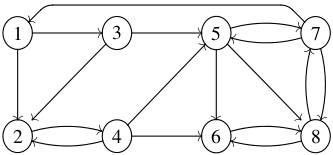
\includegraphics[width=0.4\textwidth]{images/google-internet.png}
    \caption{Beispiel-Internet mit 8 Knoten}
    \label{fig:awesome_image}
\end{figure}

Ereignisse:
\begin{itemize}
\item $S_{i}$ = Surfer liest Seite $i$ ($P(S_i)$ misst Beliebtheit der Seite $S_i$)
\item $S_{j}'$ = Surfer liest Seite $j$ nachdem er geklickt hat.
\end{itemize}

Aus dem Satz der Totalen Wahrscheinlichtkeit folgt
$$P(S_j') = \sum_{i=1}^N P(S_j' | S_i) \cdot P(S_i)$$

Da die Anzahl Besucher pro Webseite vor und nach einem Klick ungefähr gleich bleibt können wir $P(S_j') = P(S_j)$ gleichsetzen. Dies ergibt ein Gleichungssystem (eine Gleichung pro Webseite).

$$H = 
\begin{matrix}
  S_1 & S_2 & S_3 & S_4 & S_5 & S_6 & S_7 & S_8 &  \\
  0 & 0 & 0 & 0 & 0 & 0 & \frac{1}{3} & 0 & S_1' \\
  \frac{1}{2} & 0 & \frac{1}{2} & \frac{1}{3} & 0 & 0 & 0 & 0 & S_2' \\
  \frac{1}{2} & 0 & 0 & 0 & 0 & 0 & 0 & 0 & S_3' \\
  0 & 1 & 0 & 0 & 0 & 0 & 0 & 0 & S_4' \\
  0 & 0 & \frac{1}{2} & \frac{1}{3} & 0 & 0 & \frac{1}{3} & 0 & S_5' \\
  0 & 0 & 0 & \frac{1}{3} & \frac{1}{2} & 0 & 0 & \frac{1}{2} & S_6' \\
  0 & 0 & 0 & 0 & \frac{1}{2} & 0 & 0 & \frac{1}{2} & S_7' \\
  0 & 0 & 0 & 0 & 0 & 1 & \frac{1}{3} & 0 & S_8' 
\end{matrix}$$


\begin{align*}
P(S_{j}') &= \sum\limits{i=1}^N P(S_{j}'|S_{i}) \cdot P(S_{i}) \\
P(S_{j}'|S_{i}) &= \text{Zeile von } H \\
\text{mit } p = \begin{pmatrix}
\dots \\
P(S_{j}) \\
\dots
\end{pmatrix},\quad p' &= Hp
\end{align*}

Mit der Zeit stabilisieren sich die Wahrscheinlichkeiten $P(S_i)$ und $p$ konvergiert zum Eigenvektor mit Eigenwert 1 von $H$.

\subsubsection{Berechnung des Eigenwertes}
$H$ ist eine sehr spezielle Matrix. Alle Spalten summieren zu $1$ auf, und alle anderen Eigenwerte sind kleiner als $1$.

\begin{align*}
p &= a_pp + a_1v_1 + a_2v_2 + \dots \\
H^np &= a_pp + a_1\lambda_1^nv_1 + a_2\lambda_2^nv_2 + \dots \\
\Rightarrow H^np &=a_pp
\end{align*}

Da die $\lambda_i$ alle kleiner als 1 sind verschwinden diese Terme mit grösseren $n$, und übrig bleibt $p$

\subsubsection{Freier Wille}
F: Surfer setzt freien Wille ein. $P(F) = 1 - \alpha$ (Konfigurationsparameter).

\begin{align*}
P(S_{j}') & = P(S_{j}'|F)\cdot P(F) + P(S_{j}'|\bar{F})\cdot P(\bar{F}) \\
\Rightarrow p & = \frac{1}{N}\cdot (1-\alpha) +  \alpha Hp
\end{align*}

G ist die Google-Matrix, A ist eine Matrix voller Einsen.
$$
p = Gp = \alpha Hp + (1-\alpha)\frac{1}{N}Ap \rightarrow G = \alpha H + (1-\alpha)\frac{1}{N}A 
$$
\fi

\section{Zufallsvariablen, Erwartungswert, Varianz}

\subsection{Zufallsvariablen}

Ereignisse treffen ein oder nicht. Wir wollen Versuchsausgängen aber einen Wert zuweisen können.
Beim Würfeln haben wir die unterschiedlichen Bilder auf den Würfel-Seiten als Wert interpretiert, d.h. wir haben implizit eine Funktion 
$$X: \Omega \rightarrow \mathbb{R}\ :\ \omega \rightarrow X(\omega)$$

$X$ ist eine Zufallsvariable (ZV). Diese Zufallsvariable definiert nun neue Ereignisse:
\begin{align*}
\{ X = x \} \quad& P(X = x) \\
\{ X \le a \} \quad& P(X\le a) \\
\{ X > a \} \quad& P(X > a)
\end{align*}

\subsection{Erwartungswert}
$X$ ist eine Zufallsvariable.

$$E(X) = \sum_{\text{Werte}} \text{Wert} \cdot \text{Wahrscheinlichkeit} = \sum_{i=1}^n x_i \cdot P(X = x_i) $$

\ifincludeExamples
\begin{center}
\begin{tabular}{c | c | c} 
Werte & Wahrscheinlichkeit \\ \hline
1 & $\frac{1}{6}$ & $1 \cdot \frac{1}{6}$ \\
2 & $\frac{1}{6}$ & $2 \cdot \frac{1}{6}$ \\
3 & $\frac{1}{6}$ & $3 \cdot \frac{1}{6}$ \\
4 & $\frac{1}{6}$ & $4 \cdot \frac{1}{6}$ \\
5 & $\frac{1}{6}$ & $5 \cdot \frac{1}{6}$ \\
6 & $\frac{1}{6}$ & $6 \cdot \frac{1}{6}$ \\ \cline{3-3}
\multicolumn{2}{c|}{} & $\frac{21}{6} = 3.5$  
\end{tabular}
\end{center} 

Intuition: Erwartungswert $E(X)$ verhält sich wie ein Integral $\int f(x) dx$.
\fi

\subsubsection{Rechenregeln für Erwartungswerte $E(\ .\ )$}

$E(\ .\ )$ ist eine lineare Funktion.
\begin{align*}
\text{Add. Linearität: } & E(X+Y) = E(X) + E(Y) \\
\text{Mult. Linearität: } & E(\lambda X) = \sum_{i=1}^n \lambda x_i P(X = x_i) = \lambda \sum_{i=1}^n x_i P(X = x_i) \\
X \text{ und } Y \text{ unabhängig } &\Longleftrightarrow \forall x,y: \{ X = x \} \text{ und } \{Y = y\} \implies E(XY) = E(X)E(Y)
\end{align*}

\subsection{Varianz}
Varianz ist die Abweichung nach ``links'' und ``rechts''. Intuitiv: $X - E(X)$. Aber:
$$ E(X - E(X)) = E(X) - E(E(X)) = E(X) - E(X) = 0 $$
Die negativen Vorzeichen stellen ein Problem dar. Da Beträge aus analytischer Sicht suboptimal sind (Nullpunkt) ist die Lösung die Quadratfunktion.

\begin{align*}
 \text{Varianz } \var(X) &= E((X - E(X))^2) \\
 \text{Einfachere Formel: } \var(X) &= E(X^2 - 2XE(X) + E(X)^2) \\
  & = E(X^2) - 2E(X)E(X) + E(X)^2 \\
  & = E(X^2) - E(X)^2
\end{align*}

\ifincludeExamples
\subsubsection{Beispiel}
\begin{center}
\begin{tabular}{c | c | c | c | c}
X & P & $X^2$     & $X \cdot P(X)$ & $X^2 \cdot P(X)$ \\ \hline
1 & $\frac{1}{6}$ & 1  & $\frac{1}{6}$ & $\frac{1}{6}$ \\
2 & $\frac{1}{6}$ & 4  & $\frac{2}{6}$ & $\frac{4}{6}$ \\
3 & $\frac{1}{6}$ & 9  & $\frac{3}{6}$ & $\frac{9}{6}$ \\
4 & $\frac{1}{6}$ & 16 & $\frac{4}{6}$ & $\frac{16}{6}$ \\
5 & $\frac{1}{6}$ & 25 & $\frac{5}{6}$ & $\frac{25}{6}$ \\
6 & $\frac{1}{6}$ & 36 & $\frac{6}{6}$ & $\frac{36}{6}$ 
\end{tabular}
\end{center}

\begin{align*}
E(X) &= \frac{21}{6} = \frac{7}{2}, \quad E(X^2) = \frac{91}{6} \\
\var(X) & = E(X^2) - E(X)^2 = \frac{91}{6} - \frac{49}{4} = \frac{35}{12} \\
\sqrt{\var(X)} &\approx 1.707 \\
\end{align*}
\fi

\subsubsection{Rechenregeln für Varianz}
\begin{align*}
\var(\lambda X) & = E((\lambda X)^2) - E(\lambda X)^2  = \lambda^2 E(X^2) - \lambda^2E(X)^2 \\
               & = \lambda^2 \var(X) \\
\var(X+Y)       & = E((X+Y)^2) - E(X+Y)^2 \\
               & = E(X^2) + 2E(XY) + E(Y^2) - E(X^2) - 2E(X)E(Y) - E(Y^2) \\
               & = \var(X) + \var(Y) + 2(\underbrace{E(XY) - E(X)E(Y)}_{\cov(X, Y)}) 
\end{align*}

$\cov$ ist die Kovarianz, welche ist 0 wenn $X$ und $Y$ unabhängig sind.

\subsection{Genauigkeit des Mittelwertes}
$X$: Zufallsvariable, $\mu = E(X)$, $\,\varepsilon$: erwünschte Genauigkeit. \\
Gesucht: $ P(|X - \mu| > \,\varepsilon) $
 
\begin{itemize}
\item $\,\varepsilon \text{ klein } \Rightarrow P (|X-\mu| > \,\varepsilon) \text{ gross}$.
\item $\var(X) \text{ grösser } \Rightarrow P (|X-\mu| > \,\varepsilon) \text{ grösser}$.
\end{itemize}

\subsubsection{Satz von Tschebyscheff}
 $$P (|X-\mu| > \,\varepsilon) \le \frac{\var(X)}{\,\varepsilon^2}$$
\ifincludeExamples
\subsubsection{Beweis}
\begin{align*}
\text{Ereignis } A &= \{ |X-\mu| > \,\varepsilon \} \\
\text{besondere ZV: } \chi_A & = \begin{cases}1 & \quad A \text{ eingetreten} \\ 
                                              0 & \quad \text{sonst}
                                 \end{cases} & \text{logischerweise: } \chi^2 = \chi\\
E(\chi_A) & = 0\cdot P(\chi_A = 0) + 1\cdot P(\chi_A = 1) = P(A) \\
\varepsilon &\le |X - \mu| & \text{gilt falls } A \text{ eingetreten} \\
\varepsilon \chi_A &\le |X-\mu| & ()^2 \text{ statt Betrag} \\
\varepsilon^2\chi_A^{\cancel{2}} &\le (X-\mu)^2 & |\ E(\ .\ ) \\
\varepsilon^2P(A) = \,\varepsilon^2E(\chi_A)&\le E((X-E(X))^2) = \var(X) \\
\varepsilon^2P(|X-\mu|>\,\varepsilon) & \le \var(X)
\end{align*}
\fi

\subsubsection{Genauigkeit erhöhen}
Viele Messungen $X_1, X_2, \dots, X_n$. $ \text{Mittelwert } M_n = \frac{X_1+ X_2+ \dots + X_n}{n}$ wird \emph{genauer} mit mehr Messungen.

\begin{align*}
E(M_n) & = E\left( \frac{X_1+ X_2+ \dots + X_n}{n}\right)  \\
& = \frac{E(X_1) + E(X_2) + \dots + E(X_n)}{n} \\
& = E(X) \\
\var(M_n) &= var\left(\frac{X_1+ X_2+ \dots + X_n}{n}\right) \\
&\stackrel{\text{falls }X_i\text{ unabhängig}}{=} \frac{\var(X_1)+ \var(X_2)+ \dots + \var(X_n)}{n^2} \\ % FIXME text should be above =
& = \frac{n\cdot \var(X)}{n^2} \\
& = \frac{\var(X)}{n}
\end{align*}
Die Varianz wird also kleiner bei mehr \emph{unabhängigen} Messungen.

$$ P(|M_n - \mu| > \,\varepsilon) \le \frac{\var(M_n)}{\,\varepsilon^2} = \frac{\var(X)}{n\,\varepsilon^2} $$
Erwartungswert und Varianz lassen sich nun wie folgt ausdrücken:
\begin{align*}
E(X) & = \lim_{n\to\infty} \frac{1}{n} \sum_{i=1}^n x_i \\
\var(X) & = \frac{1}{n} \sum_{i=1}^n x_i^2 - \left(\frac{1}{n} \sum_{i=1}^n x_i\right)^2
\end{align*}
Je mehr Messungen vorhanden sind, desto weniger wahrscheinlich ist eine Abweichung grösser als $\,\varepsilon$ (\emph{Gesetz der grossen Zahlen}).

Falls $P(|M_n - \mu| > \,\varepsilon) \le p$ sein soll:
\begin{align*}
  p & \le \frac{\var(X)}{n\,\varepsilon^2} \quad\Rightarrow\quad
  n \le \frac{\var(X)}{p\,\varepsilon^2} \\
  \text{worst case: } n &= \frac{\var(X)}{p\,\varepsilon^2} \quad {d.h.}\quad n \sim \frac{1}{\,\varepsilon^2}
\end{align*}

\subsection{Wie genau ist die Häufigkeit als Mass für die Wahrscheinlichkeit?}
Ereignis $A$ mit Wahrscheinlichkeit $P(A)$.

\begin{align*}
  h_n = \frac{\text{Anzahl eingetreten}}{n} & & P(|h_n - P(A)| > \,\varepsilon) =\text{ ?} \\% P(A) = E(\chi_A), \chi_A = X
h_n = \frac{X_1 + X_2 + \dots + X_n}{n} = M_n& & P(|M_n - \mu| > \,\varepsilon) \le \frac{\var(\chi_A)}{n\,\varepsilon^2} 
\end{align*}

\begin{align*}
\var(\chi_A) & = E(\chi_A^{\cancel{2}}) - E(\chi_A)^2 \\
& = P(A) - P(A)^2 \\
& = P(A) (1 - P(A)) \\
P(|h_n - P(A)| > \,\varepsilon) & \le \frac{P(A)(1-P(A))}{n\,\varepsilon^2} \le \frac{1}{4n\,\varepsilon^2} \qquad(\text{da } x(1-x) \le \frac{1}{4})
\end{align*}

\subsection{Anwendung: Lineare Regression}
Zwei Zufallsvariablen $X$, $Y$, mit $Y\approx aX+b$. Das Ziel ist, für Messungen $x_i, y_i$ bestmögliche $a$ und $b$ zu ermitteln.

\ifincludeExamples
\paragraph{Beispiel: Wie lange muss ein Verzögerungselement sein?}

\begin{itemize}
\item Konstante Abbrand-Geschwindigkeit, d.h. linearer Zusammenhang zwischen Länge und Brenndauer. $$L = aT + b$$
\end{itemize}

Gesucht ist nun $L = aT + b + Fehler$ mit möglichst kleinem Fehler.
\fi

\paragraph{Problem} Finde $a$, $b$ so, dass $Y-aX-b$ minimal.
\paragraph{Gesucht}
\begin{enumerate}
\item Im Mittel kein Fehler: $E(Y - aX-b) = E(Y) - aE(X) - b = 0$
\item Möglichst kleine Varianz: $var(Y - aX - b)$ minimal
\end{enumerate}

\ifincludeDerivations
Das ist ein Optimierungsproblem. Idee: Ableiten.
\begin{align*}
  \var(Y - aX - b) &= E((Y-aX-b)^2) - E(Y-aX-b)^2 \\ 
                   &= E(Y^2) + a^2E(X^2) + \cancel{b^2} - 2aE(XY) - \cancel{2bE(Y)} + \cancel{2abE(X)} - \\
                   &  \quad \left(E(Y)^2 + a^2E(X)^2 + \cancel{b^2} - 2aE(X)E(Y) - \cancel{2bE(Y)} + \cancel{2abE(X)}\right) \\
                   &=  \var(Y) + a^2\var(X) - 2a\cov(X, Y) = Q\\[0.2cm]
  \frac{\partial Q}{\partial a} &= 2a\var(X) - 2\cov(X, Y) = 0
\end{align*}
\fi
\begin{align*}
                   a &= \frac{\cov(X, Y)}{\var(X)} \\
                   b &= E(Y) - aE(X)
\end{align*}

%Alternativer Weg: 
%\begin{align*}
%  Q & = E(Y^2) + a^2E(X^2) + b^2 - 2aE(XY) - 2bE(Y) + 2abE(X) \\
%  \frac{\partial Q}{\partial a} &= 2aE(X^2) - 2E(XY) + 2bE(X) = 0 \\
%  \frac{\partial Q}{\partial b} &= 2b - 2E(Y) + 2aE(X) = 0 \\
%  E(X^2)a + E(X)b & = E(XY) \\
%  E(X)a + b & = E(Y)
%\end{align*}
%\begin{align*}
%  a &= \begin{array}{c}\left[\begin{array}{cc}E(XY) & E(X) \\ E(Y) & 1\end{array}\right] \\ \hline  %FIXME
%                       \left[\begin{array}{cc}E(X^2) & E(X) \\ E(X) & 1\end{array}\right]\end{array} & \text{ Kramersche Regel}\\
%  & = \frac{E(XY) - E(X)E(Y)}{E(X^2)-E(X)^2} = \frac{\cov(X, Y)}{\var(X)}
%\end{align*}

Link zu Messdaten:

\begin{align*}
\text{Mittelwert: } \qquad E(X) & = \frac{1}{n}\sum_{i=1}^n x_i \\
                              a & = \frac{\frac{1}{n}\sum_{i=1}^n x_iy_i - \frac{1}{n^2}\sum_{i=1}^n x_i\sum_{j=1}^n y_j}{\frac{1}{n}\sum_{i=1}^n x_i^2 - \left(\frac{1}{n}\sum_{j=1}^n x_i\right)^2} \\
                              b & = E(Y) - aE(X) = \frac{1}{n}\sum_{i=1}^n x_i - a\frac{1}{n}\sum_{i=1}^n y_i
\end{align*}

Diese Formeln zeigen uns, dass es möglich ist, lineare Regression durchzuführen ohne grosse Speicher zu benötigen.

\subsection{Qualitätsmass für die Approximation}
Idee: $var(Y-aX-b)$ ``klein'' bedeutet gut, ``gross'' schlecht. Problem: Masseinheiten.

\begin{align*}
\var(Y-aX-b) & = \var(Y) + a^2\var(X) - 2a\cov(X, Y) & \text{ aber wir kennen jetzt } a\\
             & = \var(Y) + \frac{\cov(X, Y)^2}{\var(X)^{\cancel{2}}}\cancel{\var(X)} - 2\frac{\cov(X, Y)}{\var(X)} \cov(X,Y) \\
             & = \var(Y) - \frac{\cov(X, Y)^2}{\var(X)}\\
             & = \var(Y) \underbrace{\left(1 - \frac{\cov(X,Y)^2}{\var(X)\var(Y)}\right)}_{\text{dimensionslos}}
\end{align*}
Daraus können wir ableiten:
\begin{align*}
\text{``gut''} & \Leftrightarrow 1 - \frac{\cov(X,Y)^2}{\var(X)\var(Y)} \text{ klein} \\
               \Rightarrow \text{ Regressionskoeffizient } r^2 & = \frac{\cov(X,Y)^2}{\var(X)\var(Y)} \text{ nahe bei } 1 \\
\text{``schlecht''} & \Leftrightarrow r^2 = \frac{\cov(X,Y)^2}{\var(X)\var(Y)} \text{ nahe bei } 0 \text{ (Unabhängigkeit)} \\
r & := \frac{\cov(X,Y)}{\sqrt{\var(X)\var(Y)}}
\end{align*}
$r$ erlaubt uns, 3 Fälle zu unterscheiden:
\begin{description}
\item[$r\sim 0$] Punkte sind grösstenteils unabhängig voneinander (schlechtes Resultat)
\item[$r\sim 1$] Punkte sind abhängig voneinander (positive Korrelation), auf einer steigenden Geraden
\item[$r\sim -1$] Punkte sind abhängig voneinander (negative Korrelation), auf einer abfallenden Geraden
\end{description}

\section{Verteilungsfunktionen}
Die bisherige Vorgehensweise funktioniert gut für diskrete Zufallsvariablen mit wenigen Werten, stösst jedoch auf Probleme bei unendlich vielen, oder stetig verteilten (reelle Zahlen) Werten. Ausserdem mussten wir bisher genau wissen, wie $\Omega$ aussieht (dies erlaubte auch das Rechnen mit abhängigen Variablen).

\subsection{Definition}
Gesucht ist eine Funktion, welche alle relevanten Wahrscheinlichkeitsinformationen codiert:
$$X \leadsto F_X(x)$$

Ereignisse, die zu X gehören:
\begin{align*}
 \{X = a\} &  \leadsto P(X= a) = F_X(x) - \lim_{\varepsilon\to x-} F_X(\varepsilon) \\
 \{X\le a\} &  \leadsto P(X\le a) =: F_X(a) \\
 \{a < X \le b\} & \leadsto P(a < X \le b) = F(b) - F(a) 
\end{align*}

\ifincludeExamples
\paragraph{Beispiel} $X = $ ``Würfel''
$$ F_X(a) = \text{ Wahrscheinlichkeit, dass Augenzahl } \le a = P(x \le a) $$ % F_X(a) springt stufenweise 

Von der Verteilungsfunktion zur Wahrscheinlichkeit:
\begin{align*}
P(X=2) & = P(1.5 < X \le 2.5) = P(X\le2.5) - P(X\le1.5) = F(2.5) - F(1.5) \\
\text{besser } P(X=2) & = F(2) - \lim_{x\to2-} F(x)
\end{align*}

\paragraph{Beispiel: $\infty$ -Würfel}
Zylinder mit Endposition $X$ in $[0, 2\pi]$
\begin{align*}
P(a<X\le b) & = \frac{b-a}{2\pi} \\
F(a) = P(X\le a) & = P(0<X\le a) = \frac{a}{2\pi}
\end{align*}
\fi
\subsection{Eigenschaften von Verteilungsfunktionen}
\begin{align}
0 & \le F(x) \le 1 \\
x_1 \le x_2 & \Rightarrow F(x_1) \le F(x_2) & \text{ monoton steigend} \\
\lim_{x\to-\infty} F(x) = 0, & \quad\lim_{x\to\infty} F(x) = 1
\end{align}

\subsection{Erwartungswert}

Bisher haben wir den Erwartungswert wie folgt definiert:
$$
  E(X) = \sum_{\text{Werte}} \text{ Wert } \cdot \text{ Wahrscheinlichkeit }
$$

Problem: Unabzählbar viele Werte!

\begin{align*}
E(X) & = \sum_i x_i \cdot P(x_i < X \le x_{i+1}) \\
     & = \sum_i x_i \cdot \left(F(x_{i+1}) - F(x_i)\right) \\
     & = \sum_i x_i \cdot \left(F(x_{i+1}) - F(x_i)\right) \cdot \frac{x_{i+1} - x_i}{x_{i+1} - x_i} \\
     & = \sum_i x_i \cdot \underbrace{\frac{F(x_{i+1}) - F(x_i)}{x_{i+1} - x_i}}_{\text{mit} \Delta x \to 0 \text{: Ableitung}} x_{i+1} - x_i \\
\rightarrow  E(X) & = \int_{-\infty}^\infty x\cdot F'_X(x) dx = \int_{-\infty}^\infty x\cdot \varphi(x) dx \\
F_X'(x) & = \varphi_X (x)\text{ Wahrscheinlichkeit, Dichtefunktion} \\
F_X & = \text{ Stammfunktion von } \varphi_X = \int_{-\infty}^x \varphi_X(\xi)d\xi \\
P(a<X\le b) & = F_X(b) - F_X(a) = \int_a^b \varphi_X(x) dx
\end{align*}

\ifincludeExamples
\paragraph{Beispiel $\infty$-Würfel}
\begin{align*}
E(X) & = \int_{-\infty}^\infty x\cdot F'_X(x) dx & \text{F(x) ist } 0 \text{ links und rechts von } 0/2\pi \\
     & = \int_{-0}^{2\pi} x\cdot \frac{1}{2\pi} dx \\
     & = \left[ \frac{1}{4\pi} x^2\right]_0^{2\pi} = \frac{4\pi^2}{4\pi} = \pi 
\end{align*}
\fi

\subsection{Varianz}
\begin{align*}
\var(X) = E(X^2) - E(X)^2 \\
E(X^2) = \int_{-\infty}^\infty \underbrace{x^2}_{\text{Wert}}\qquad\cdot\underbrace{\varphi_X(x)}_{\text{Wahrscheinlichkeit}} dx \\
\end{align*}

\ifincludeExamples
\paragraph{Beispiel $\infty$-Würfel}
\begin{align*}
E(X^2) & = \int_{-\infty}^\infty x^2 \varphi_X(x) dx = \int_{-\infty}^\infty x^2 \frac{1}{2\pi} dx 
         = \left[\frac{x^3}{6\pi}\right]_0^{2\pi} = \frac{8\pi^3}{6\pi} = \frac{4}{3}\pi^2 \\
\var(X) & = E(X^2) - E(X)^2 = \frac{4}{3}\pi^2 - \pi^2 = \frac{1}{3}\pi^2, stddev = \frac{1}{\sqrt{3}}\pi = 0.58\pi
\end{align*}
\fi

\subsection{Eigenschaften der Dichtefunktion $\varphi_X$ } % folgen aus Eigenschaften von F_X
\begin{align}
F_X \text{ monoton wachsend } &\Rightarrow \quad\varphi_X(x) = F_X'(x) \ge 0 \\
F_X(x) \to 1 \text{ für } x\to \infty &\Rightarrow \int_{-\infty}^\infty \varphi_X(x) dx 
  = \lim_{a\to\infty} \underbrace{\int_{-\infty}^a\varphi_X(x) dx}_{F_X(a)} = 1
\end{align}

\ifincludeExamples
\begin{align*}
\varphi(x) = \begin{cases}a\cos x & -\frac{\pi}{2} \le x \frac{\pi}{2} \\ 0 & \text{ sonst}\end{cases} \\
\varphi(x) \ge 0 & \forall x\in\mathbb{R} \text{ ok} \\
\int_{-\infty}^\infty \varphi(x) dx = \int_{-\frac{\pi}{2}}^\frac{\pi}{2} a\cos x dx = a\left[sin x\right]_{-\frac{\pi}{2}}^\frac{\pi}{2} = 2a
\end{align*}
Also eine gültige Dichtefunktion für $a=\frac{1}{2}$
\begin{align*}
F(X) = \int_{-\infty}^x \varphi(\xi)d\xi = \int_{-\frac{\pi}{2}}^x \frac{1}{2}\cos\xi d\xi = \frac{1}{2}\left(sin(x) + 1\right)
\end{align*}
\fi

\subsection{Berechnung von Varianten} % TODO: fix title
Algorithmus am Beispiel von $F_{X^2}$, $\varphi_{X^2}$:
\begin{align*}
F_{X^2} & = P(X^2 \le x) & \text{Definition verwenden}\\
        & = P(|X| \le \sqrt{x}) & \text{Umformen auf } P(X \le \dots) \\
        & = P(-\sqrt{x} \le X \le \sqrt{x}) \\
        & = F_X(\sqrt{x}) - F_X(-\sqrt{x}) & \text{Definition von } F_X\text{ anwenden} \\
\varphi_{X^2} & = \frac{d}{dX} F_{X^2}(x) = \frac{d}{dX}\left(F_X(\sqrt{x}) - F_X(-\sqrt{x}\right) \\
        & = F'_X(\sqrt{x}) \frac{1}{2\sqrt{x}} + F'_X(-\sqrt{x}) \frac{1}{2\sqrt{x}} \\
        & = \frac{1}{2\sqrt{x}} \left( F'_X(\sqrt{x}) + F'_X(-\sqrt{x})\right) \\
        & = \frac{1}{2\sqrt{x}} \left(\varphi_X(\sqrt{x}) + \varphi_X(-\sqrt{x})\right) \\[1cm]
F_{\sqrt{X}} & = P(\sqrt{X} \le x) \stackrel{X\ge0}{=} P(X \le x^2) \\
             & = F_X(x^2) \\
\varphi_{\sqrt{X}} & = \frac{d}{dx} F_{\sqrt{X}}(x) = \frac{d}{dx} F_X(x^2) = 2x \cdot F_X(x^2) = 2x\cdot\varphi_X(x^2)
\end{align*}
\begin{align*}
F_{\lambda X}(x) & = P(\lambda X \le x) = P\left(X \le \frac{x}{\lambda}\right) & \lambda > 0 \\
                 & = F_X\left(\frac{x}{\lambda}\right) \\
\varphi_{\lambda X}(x) & = \frac{d}{dx}F_{\lambda X}(x) = \frac{d}{dx}F_{X}\left(\frac{x}{\lambda}\right) \\
                       & = F'_X\left(\frac{x}{\lambda}\right) \frac{1}{\lambda} = \varphi_X\left(\frac{x}{\lambda}\right)\frac{1}{\lambda} \\
E(\lambda X) & = \int_{-\infty}^\infty x\varphi_{\lambda X} (x)dx \\
             & = \lambda\int_{-\infty}^\infty \underbrace{\frac{x}{\lambda}}_z \varphi_X(\underbrace{\frac{x}{\lambda}}_z) \underbrace{\frac{dx}{\lambda}}_{dz} \\
             & = \lambda \int_{-\infty}^\infty z\varphi_X(z) dz = \lambda E(X)
\end{align*}

Annahme: $X$, $Y$ unabhängig.
\begin{align*}
\varphi_{X+Y}(s) \cdot \Delta s & = \text{ Wahrscheinlichkeit, dass } X+Y \text{ in einem Interval } \Delta s \text{ um } s \text{ liegt} \\
 & = \underbrace{\text{ Wahrscheinlichkeit, dass } X \text{ in einem Interval um } x \text{ liegt }}_{\varphi_X(x) \cdot \text{ Interval}} \wedge \\& \qquad\underbrace{\text{ dass } Y \text{ in einem Interval um } s-x}_{\varphi_Y(s-x)\cdot \text{ Interval}} \underbrace{\text{ für alle } x-\text{ Intervalle liegt}}_{\rightarrow Summe} \\
  &= \int_{-\infty}^\infty \varphi_X(x) \varphi_Y(s-x) dx \Delta s \\
  \Rightarrow \varphi_{X+Y}(s) & = \int_{-\infty}^\infty \varphi_X(x) \varphi_Y(s-x) dx = \varphi_X *\ \varphi_Y(s) = \text{ Faltung}
\end{align*}

\ifincludeExamples
Beispiel mit $X$, $Y$ gleichverteilt in [0,1]:
\begin{align*}
\varphi_X(x) & = \begin{cases} 0 & x \le 0 \\ 1 & 0 < x \le 1 \\ 0 & x > 1\end{cases}\\
\varphi_{Y}(s-x) & = \begin{cases}0 & s-x> 1 \Leftrightarrow x < s-1 \\ 1 & s-1\le x < s \\ 0 & x\ge s\end{cases} \\
\varphi_{X+Y} (s) & = \int_{-\infty}^\infty \varphi_X(x)\varphi_Y(s-x) dx & \varphi_X(x) \text{ ist immer 1 im relevanten Bereich}\\
                  & = \int_0^1 \varphi_Y(s-x) dx \\
\varphi_{X+Y}(s) & = \begin{cases} 0 & s < 0 \\ s & 0\le s <1 \\1-(s-1) = 2-s & 1 \le s \le 2\\ 0 & s > 2 \end{cases} \\
\end{align*}
\fi

\subsection{Erzeugung von Zufallszahlen mit Verteilungsfunktion $F$}
\begin{description}
\item[Gegeben] Zufallsvariable $X$ mit Verteilungsfunktion $F$, Y = F(X), Y ist ZV mit Werten in [0, 1].
\item[Gesucht] $F_Y$
\end{description}

\begin{align*}
  F_Y(y) & \stackrel{\text{Def}}{=} P(Y \le y) \\
         & = P(F(X) \le y)  & F \text{ umkehrbar da monoton wachsend} \\
         & = P(X \le F^{-1}(y)) \\
         & \stackrel{\text{Def}}{=} F(F^{-1}(y)) = y 
\end{align*}

$F(X)$ ist also gleichverteilt!
Umgekehrt: $Y$ gleichverteilt $\Rightarrow F^{-1}(Y)$ hat Verteilungsfunktion $F$.

\section{Katalog von Wahrscheinlichkeitsverteilungen}
\newlength{\katalogSpaltezwei}
\setlength{\katalogSpaltezwei}{11.5cm}

\subsection{Gleichverteilung in Intervall $[\,a, b\,]$}
\begin{tabular}{r p{\katalogSpaltezwei}}
Anwendung & Zufallszahlen \\
Dichtefunktion & $\varphi(x) = \begin{cases}\frac{1}{b-a} & a < x < b \\ 0 & \text{sonst} \end{cases} $ \\
Verteilungsfunktion & $F(x) = \begin{cases}0 & x < a \\ \frac{x-a}{b-a} & a < x < b \\ 1 & x > b\end{cases} $ \\
Erwartungswert & $E(X) = \frac{a+b}{2}$ \\
Varianz & $\var(X) = \frac{(b-a)^2}{12}$ \\
Median & $ \median(X) = \frac{a+b}{2} $ \\
Abweichungen & $P(|X - E(X)| > \varepsilon) = 1 - \frac{2\epsilon}{b-a}$ für $\varepsilon < \frac{b-a}{2}$
\end{tabular}

\subsection{Exponentialverteilung}
\begin{tabular}{r p{\katalogSpaltezwei}}
Anwendung & Zeitabhängige Prozesse ohne Erinnerungsvermögen (ungesättigte Queues, 
            Ausfall von Hardware ohne Alterungsprozess, radioaktiver Zerfall) \\
Dichtefunktion & $\varphi(x) = \begin{cases} 0 & x < 0 \\ \frac{1}{a}e^{-ax} & x \ge 0 \end{cases} $ \\
Verteilungsfunktion & $F(x) = \begin{cases} 0 & x<0 \\ 1 - e^{-ax} & x \ge 0 \end{cases} $ \\
Erwartungswert & $E(X) = \frac{1}{a} $ \\
Varianz & $\var(X) = \frac{1}{a^2} $ \\
Median & $ \median(X) = \frac{1}{a} \log 2 \approx \frac{1}{a} 0.693 $ \\
Abweichungen & $P(|X - E(X)| > \varepsilon) = \begin{cases} e^{-a\varepsilon-1} & \varepsilon > \frac{1}{a} \\ 1 - e^{a\varepsilon-1} + e^{-a\varepsilon-1} & \varepsilon \le \frac{1}{a}\end{cases}$ 
\end{tabular} 

$\frac{1}{a}$ ist die mittlere Zeit zwischen 2 Ereignissen (z.B. MTBF bei Hardware).

\ifincludeDerivations
\subsubsection{Herleitung}
\begin{align*}
\text{kein Erinnerungsvermögen}: P(X\le t) & = P(X \le t + t_0 | X > t_0) \\ 
1 - F(t) & = P(X>t) = g(t) \\
P(X>t) & = P(X > t+t_0 | X > t_0) & \text{mit } P(A|B) = \frac{P(A\cap B)}{P(B)}\\ 
 & =  \frac{P(X > t+t_0 \wedge \cancel{X > t_0})}{P(X>t_0)} \\ 
 & = \frac{P(X > t+t_0)}{P(X>t_0)} \\
 & = \frac{g(t+t_0)}{g(t_0)} \\
 \text{Funktionalgleichungen } g(t+t_0) & = g(t)g(t_0) & \text{``Lösung durch Anstarren'': } e^x\\
\end{align*}
Wir dürfen aus der Konstruktion annehmen, dass $g'$ existiert.
\begin{align*}
\text{Ableiten nach} t_0: g'(t+t_0) & = g(t)g't(t_0) \\
\lim_{t_0 \to 0} g'(t) & = g(t)g'(0) & \text{DGL für } g \\
\Rightarrow g(t) & = e^{-at} 
\end{align*}

\begin{align*}
E(X) & = \int_{-\infty}^\infty t\,\varphi(t)\,dt = \int_0^\infty t\,ae^{-at}\,dt & \rightarrow \text{ Partielle Integration} \\
     & = \underbrace{\left[ ta\frac{1}{-a}e^{-at}\right]_0^\infty}_{\to 0} - \int_0^\infty 1\frac{1}{-a}ae^{0at}dt \\
     & = \int_0^\infty e^{-at} dt = \left[ \frac{1}{-a}e^{-at}\right]_0^\infty \\
     & = 0 - \frac{1}{-a} = \frac{1}{a}
\end{align*}
Wahrscheinlichkeit, dass ein Ereignis früher als erwartet eintrifft:
$$ P\left(X\le\frac{1}{a}\right) = F\left(\frac{1}{a}\right) = 1-e^{-1} = 0.6321 $$
\begin{align*}
E(X^2) & = \int_{-\infty}^\infty t^2\,\varphi(t)\,dt = \int_0^\infty t^2\,ae^{-at}\,dt \\
       & = \left[t^2 a\frac{1}{-a}e^{-at}\right]_0^\infty - \int_0^\infty 2t a\frac{1}{-a}e^{-at} dt \\
       & = \frac{2}{a}\int_0^\infty t\,e^{-at}\,dt = \frac{2}{a}\frac{1}{a} \\
var(X) & = E(X^2) - E(X)^2 = \frac{2}{a^2} - \left(\frac{1}{a}\right)^2 = \frac{1}{a^2}
\end{align*}

Halbwertszeit = Median:
\begin{align*}
\median(X) & = F(t_{\frac{1}{2}}) = \frac{1}{2} \\
1-e^{-at} & = \frac{1}{2} \\
\log \frac{1}{2} = -at_{\frac{1}{2}} &\Rightarrow t_{\frac{1}{2}} = \frac{1}{a} \log 2 \approx \frac{1}{a} 0.693
\end{align*}
\fi
\ifincludeExamples
\paragraph{Beispiel: Raid 1 mit 2 Disks}
Gesucht ist die Lebensdauer des Gesamtsystems.

\begin{align*}
\text{Näherung: } X_i & = \text{Lebensdauer von Disk } i \text{ exponentialverteilt, Annahme: Disks unabhängig}\\
P(\underbrace{X_1 \le t \wedge X_2 \le t}_{\text{Ereignis Totalausfall}}) & = P(X_1 \le t)\ P(X_2 \le t) \\
  & = (1-e^{-at})^2 = F_{\text{Totalausfall}}(t) \\
\varphi_{\text{Totalausfall}} & = F'(t) = 2(1-e^{-at})ae^{-at} \\
\text{Erwartete Zeit für Totalausfall: }& \int_{-\infty}^\infty t\varphi(t)dt = \int_{-\infty}^\infty t 2(1-e^{-at})ae^{-at} dt \\
 & = 2 \underbrace{\int_{-\infty}^\infty t ae^{-at} dt}_{E(X)} - \underbrace{\int_{-\infty}^\infty t 2ae^{-2at} dt}_{\text{Exponentialverteilung mit }\tilde{a} = 2a} \\
 & = \frac{2}{a} - \frac{1}{2a} = \frac{4}{2a} - \frac{1}{2a} = \frac{3}{2} \frac{1}{a} \quad \text{d.h. 50\% mehr ``Lebenserwartung''}
\end{align*}

\fi

\subsection{Poisson-Verteilung}
\begin{tabular}{r p{\katalogSpaltezwei}}
Anwendung & Anzahl Fälle eines erinnerungsfreien Ereignisses, welches mit Rate $\lambda$ eintritt, 
            Anzahl seltener Ereignisse \\
Wahrscheinlichkeit & $P_\lambda(k) = e^{-\lambda} \frac{\lambda^k}{k!}$ \\
Erwartungswert & $E(K) = \lambda $ \\
Varianz & $\var(X) = \lambda $
\end{tabular} 

\ifincludeDerivations
\subsubsection{Herleitung}
$X_1, X_2, \dots, X_n$ exponentialverteilte Zufallsvariablen, unabhängig \\
Gesucht: 
\begin{enumerate}
\item Wahrscheinlichkeit für genau $k$ Fehler-Ereignisse in Intervall $x$ \\ 
\item Erwartete Anzahl Fehler
\end{enumerate}

Dazu brauchen wir die Verteilung von $X_1 + X_2 + \dots + X_k$

\begin{align*}
\varphi_{X_1+X_2} & = \varphi_{X_1} * \varphi_{X_2} (x) = \int_{-\infty}^\infty \varphi_{X_1}(\xi) \varphi_{X_2}(x-\xi) d\xi \\ 
\varphi_k & \text{ ist Dichtefunktion von }X_1 + \dots + X_k \\
\varphi_2(x) & = \int_{-\infty}^\infty \varphi_1(\xi) \varphi_1(x-\xi) d\xi \\
& = \int_0^x ae^{-a\xi} ae^{-a(x-\xi)} d\xi \\
& = \int_0^x \underbrace{a^2e^{-ax}}_{\text{unabhängig von }\xi}\underbrace{e^{-a(\xi-\xi)}}_{1}d\xi \\
& = a^2e^{-ax} \int_0^x d\xi = a^2xe^{-ax} \\
\varphi_k(x) & = a^kx^{k-1}e^{-ax} \frac{1}{(k-1)!} & \text{ dies sind die Erlang-Verteilungen} 
\end{align*}

Wahrscheinlichkeit für genau $k$ Fehler in Zeitinterval $x$:
\begin{align*}
P(\text{genau }k) & = P(\text{mindestens } k) - P(\text{mehr als } k) \\
& = P(X_1 + \dots + X_k \le x) - P(X_1 + \dots + X_k + X_{k+1} \le x) \\
& = F_k(x) - F_{k+1}(x) \\
F_k(x) = 1 - e^{-ax}\sum_{i=0}^{k-1} \frac{(ax)^k}{i!} \\
\Rightarrow P(\text{genau k}) &= 1 - e^{-ax} \sum_{i=0}^{k-1} \frac{(ax)^k}{i!} - 
  \left(1 - e^{-ax} \sum_{i=0}^{k} \frac{(ax)^k}{i!}\right) \\
  & = e^{-ax}\frac{(ax)^k}{k!}
\end{align*}
Wichtig ist nur $ax = \lambda$.
\begin{align*}
   P(\text{genau }k) = P_{\lambda(k)} = e^{-\lambda} \frac{\lambda^k}{k!} \quad\text{Poisson-Verteilung} 
\end{align*}
\fi

\subsection{Binomialverteilung}
Ein Bernoulli-Experiment ist ein Experiment mit genau 2 möglichen Resultaten.

\begin{tabular}{r p{\katalogSpaltezwei}}
Anwendung & Wiederholte Bernoulli-Experimente \\
Wahrscheinlichkeit & $P(X=k) = \binom{n}{k} p^k(1-p)^{n-k}$ - schwierig zu berechnen für grosse $n$\\
Erwartungswert & $ E(X) = np $ \\
Varianz & $\var(X) = np\,(1-p) $ \\
Verteilungsfunktion & $F(x) = \sum_{k=0}^{k \le x} \binom{n}{k} p^k(1-p)^{n-k}$ (es gibt keine schöne Formel)
\end{tabular} 

\ifincludeDerivations
\subsubsection{Herleitung: Welche Verteilung hat die Zufallsvariable ``Anzahl Kreuze in einem Feld''?}

Das Feld hat eine Grösse von 6x6, mehrere Kreuze pro Feld sind erlaubt. Es sind 18 Kreuze zu setzen. 

Aus Sicht eines einzelnen Feldchens ist das Experiment sehr einfach: Wiederhole 18 mal das Experiment ``Kreuz mit Wahrscheinlichkeit $\frac{1}{36}$''.

Allgemein: $n$ Wiederholungen eines Bernoulli-Experiments mit Wahrscheinlichkeit $p$. Gezählt wird die Anzahl positiver Ausgänge $X$.

\begin{align*}
\text{Rechenregeln: } X_1, \dots, X_n  &\text{ unabhängige ZV der Art } \chi_A, P(A)= p \\
E(X) & = \underbrace{E(X_1)}_{p} + \dots + \underbrace{E(X_n)}_{p} = np \\
\var(X) & = \underbrace{\var(X_1)}_{p\,(1-p)} + \dots + \underbrace{\var(X_n)}_{p\,(1-p)} = np\,(1-p) \\
\text{Wahrscheinlichkeit für } &k \text{ Kreuze: } P(X = k) \\
\text{Es gibt } \binom{n}{k} &\text{ Möglichkeiten für } k \text{ positive Ausgänge} \\ 
p^k(1-p)^{n-k} &\text{ ist die Wahrscheinlichkeit für eine bestimmte Abfolge von Ausgängen} \\
\Rightarrow P(X=k) &= \binom{n}{k} p^k(1-p)^{n-k} \text{ - dies ist die Binomialverteilung.}
\end{align*}
\fi
\ifincludeDerivations
\paragraph{Berechnung des Erwartungswertes aus $P(X=k)$} 

\begin{align*}
E(X) &= \sum_{k=0}^{n} k \binom{n}{k} p^k(1-p)^{n-k} \\
     &= \sum_{k=1}^{n} \binom{n}{k} k p^{k-1}p (1-p)^{n-k} & x = p, y = p-1 \\
     &= \sum_{k=1}^{n} p \binom{n}{k} \underbrace{k x^{k-1}}_{\frac{d}{dx} x^k} y^{n-k} \\
     & = p \frac{d}{dx} \sum_{k=0}^{n} \binom{n}{k}x^k y^{n-k} \\
     & = p \frac{d}{dx} (x+y)^n \\
     & = p n (x+y)^{n-1} = pn(p + 1-p)^{n-1} \\
     & = np
\end{align*}
\fi

\subsubsection{Berechnung für grosse $n$}
Die direkte Berechnung ist schwirig für grosse $n$. Lösungsansätze:

\paragraph{Seltene Ereignisse} ``selten'' = $n$ gross, $p$ klein. Berechnung durch Poisson-Verteilung.
\ifincludeDerivations
Vermutung: Anzahl seltener Ereignisse ist Poisson-verteilt.
Beweis:
\begin{align*}
E(X) &= np = \lambda \\
\underbrace{P(X=k)}_{\text{Binomialverteilt}} & \stackrel{?}{\longrightarrow} P_\lambda(k) 
         = \frac{\lambda^k}{k!} e^{-k} \text{ für } n \to\infty \\
\binom{n}{k} p^k (1-p)^{n-k} &= \binom{n}{k} \left(\frac{\lambda}{n}\right)^k \left(1-\frac{\lambda}{n}\right)^{n-k} \\
    &= \frac{n(n-1)\cdots(n-k+1)}{1\cdot2\cdots k} \left(\frac{\lambda}{n}\right)^k 
            \left(1-\frac{\lambda}{n}\right)^n \left(1-\frac{\lambda}{n}\right)^{-k} \\
    & = \frac{\lambda^k}{k!} \underbrace{\left(1-\frac{\lambda}{n}\right)^n}_{\to e^{-\lambda}} 
             \underbrace{\left(1-\frac{\lambda}{n}\right)^{-k}}_{\to 1}
             \underbrace{\frac{n}{n}}_{\to 1} \underbrace{\frac{n-1}{n}}_{\to 1} \underbrace{\frac{n-2}{n}}_{\to 1} \cdots 
             \underbrace{\frac{n-k}{n}}_{\to 1} & \text{ mit } n\to\infty \\
    &  \to \frac{\lambda^k}{k!}e^{-\lambda} \quad \text{ für } n\to\infty
\end{align*}
\fi

\paragraph{Nicht-seltene Ereignisse ($p \approx \frac{1}{2}$)}
In diesen Fällen ist die Normalverteilung anwendbar.

\subsection{Normalverteilung, Gauss-Verteilung}
\begin{tabular}{r p{\katalogSpaltezwei}}
Anwendung & ``Summe vieler kleiner Zufallsbeiträge'', Messfehler, Brownsche Bewegung, (weisses) Rauschen \\
Dichtefunktion & $\varphi(x) = \frac{1}{\sqrt{2\pi}\sigma} e^{-\frac{(x-\mu)^2}{2\sigma^2}}$ \\
Erwartungswert & $ E(X) = \mu $ \\
Varianz & $\var(X) = \sigma^2 $
\end{tabular} 

\paragraph{Verteilungsfunktion}
\begin{align*}
F(X) = \frac{1}{\sqrt{2\pi}\sigma} \int_{-\infty}^x e^{-\frac{(\xi-\mu)^2}{2\sigma^2}} d\xi = \text{ keine ``geschlossene'' Stammfunktion}
\end{align*}


\ifincludeDerivations
Berechnung:
\begin{itemize}
\item erfinde neue Funktion: $erf(x) = \frac{2}{\pi} \int_0^x e^{-t^2}dt \Rightarrow F(x) 
         = \frac{1}{2}\left(1 + erf\left(\frac{x}{\sqrt{2}}\right)\right)$ ($\mu = 0, \sigma = 1$)
\item Tabelle
\end{itemize}

Die Tabelle hat ein Problem: Sie gilt nur für ein bestimmtes $\mu$ und $\sigma$.
Lösung: Standardisierung durch $$Z = \frac{X - \mu}{\sigma}, \mu = E(X), \sigma^2 = \var(X) \Longrightarrow E(Z) = 0, \var(Z) = 1$$ 

\subsubsection{Berechnung von $E(X), \varphi(X), \varphi_1 * \varphi_2 = \varphi_3$}
\paragraph{Warum $\frac{1}{\sqrt{2\pi}}$?}
\begin{align*}
I & = \int_{-\infty}^\infty e^{-\frac{x^2}{2}} dx = \ ? \\
I^2 & = \int_{-\infty}^\infty e^{-\frac{x^2}{2}} dx \int_{-\infty}^\infty e^{-\frac{y^2}{2}} dy \\
    & = \int \int e^{-\frac{x^2 + y^2}{2}} dx dy = \text{ Volumen unter der Fläche } z = e^{-\frac{x+y}{2}}
\end{align*}
Wechsel zu Polarkoordinaten $r, \varphi$:
\begin{align*}
z & = e^{-\frac{r^2}{2}} \\
I^2 & = \int_0^\infty \int_0^{2\pi} e^{-\frac{r^2}{2}} \underbrace{r\ d\varphi\ dr}_{\text{Grundfläche einer Säule}} \\
    & = 2\pi \int_0^\infty re^{-\frac{r^2}{2}} dr \\
    & = 2\pi \left[ -e^{-\frac{r^2}{2}} \right]_0^\infty = 2\pi (0 - (-1)) = 2\pi \\
\Rightarrow I &= \sqrt{2\pi}
\end{align*}

\paragraph{$E(X)$}
\begin{align*}
  E(X) & = \frac{1}{\sqrt{2\pi}} \int_{-\infty}^\infty xe^{-\frac{x^2}{2}} dx \\
       & = \frac{1}{\sqrt{2\pi}} \left[ -e^{-\frac{x^2}{2}} \right]_{-\infty}^\infty \\
       & = \frac{1}{\sqrt{2\pi}} (0-0) = 0
\end{align*}

\paragraph{$\var(X)$}
\begin{align*}
  \var(X) & = \frac{1}{\sqrt{2\pi}} \int_{-\infty}^\infty x^2e^{-\frac{x^2}{2}} dx \\
          & = \frac{1}{\sqrt{2\pi}} \int_{-\infty}^\infty x\cdot xe^{-\frac{x^2}{2}} dx \\
          & = \underbrace{\frac{1}{\sqrt{2\pi}} \left[ x(-e^{-\frac{x^2}{2}} \right]_{-\infty}^\infty}_{0} + 
              \underbrace{\frac{1}{\sqrt{2\pi}} \int_{-\infty}^\infty 1 e^{-\frac{x^2}{2}} dx}_{1} \\
          & = 1
\end{align*}
\fi
\subsubsection{Zentraler Grenzwertsatz}
Voraussetzungen, damit die $X_i$ vergleichbar sind.
\begin{itemize}
\item $X_1, X_2, X_3, \dots$ unabhängig
\item $E(X_i) = 0$ 
\item $\var(X_i) = 1$
\end{itemize}

\begin{align*}
    S_n & = \frac{X_1 + X_2 + \dots + X_n}{\sqrt{n}} &\Rightarrow E(S_n) = 0,\quad \var(S_n) = 1 \\
\end{align*}

$S_n$ ist eine Summe vieler kleiner Beiträge.

\ifincludeDerivations\else
Der zentrale Grenzwertsatz sagt aus, dass die Verteilungsfunktion von $S_n$ gegen die Standardnormalverteilung konvergiert.

\fi
\ifincludeDerivations

\begin{align*}
    S_n & = \frac{X_1 + X_2 + \dots + X_n}{\sqrt{n}} &\Rightarrow E(S_n) = 0,\quad \var(S_n) = 1 \\
\end{align*}

$S_n$ ist damit eine Summe vieler kleiner Beiträge.

Behauptung: Die Verteilungsfunktion von $S_n$ konvergiert gegen die Verteilungsfunktion einer Standardnormalverteilung:
Wir arbeiten mit der Dichte- statt der Verteilungsfunktion

Ziel: 
\begin{align*}
\varphi_i & = \varphi_{X_i}\\
\Asterisk_{i=1}^\infty \varphi_i & = \varphi_{\text{Normalverteilung}} % find better way to display "infinite convolution"
\end{align*}

Hilfsmittel: Momenterzeugende Funktion.
\begin{align*}
X \text{ eine ZV:} \quad M_X(t) & = E(e^{tX})
\end{align*}

Eigenschaften:
\begin{align*}
M_{\lambda X}(t) = E(e^{t(\lambda X)}) = E(e^{(\lambda t) X}) = M_X(\lambda t) \\
M_{X+Y}(t) = E(e^{t(X+Y)}) = E(e^{tX} e^{tY}) \stackrel{X,Y \text{unabh.}}{=} E(e^{tX}) E(e^{tY}) = M_X(t)M_Y(t)
\end{align*}
Die Momenterzeugende Funktion von $\varphi_X*\varphi_Y$ ist das Produkt der Momenterzeugenden Funktionen von $\varphi_X$ und $\varphi_Y$ (wie bei Fourier/Laplace-Transformation). 

Grund: 
\begin{align*}
M_X(t) = E(e^{tX}) & = \int_{-\infty}^\infty e^{tx} \varphi(x) dx & \text{ bekannt als ``beidseitige Laplace-Transformation''}
\end{align*}

Revidiertes Ziel:
\begin{align*}
M_{S_n}(t) \ &\stackrel{?}{\longrightarrow}\  M_{\text{Standardnormalverteilung}} \\
\text{Woher kommt der Name?}\qquad M_X(t) & = E(e^{tX}) = 1 + tE(X) + \frac{t^2}{2!}E(X^2) + \frac{t^3}{3!} E(X^3) + \dots \\
E(X^k) & \text{ heisst k-tes Moment von X} \\
M_X(t) &\text{ ist eine erzeugende Funktion für die Momente } E(X^k)
\end{align*}

Plan: $M_{S_n}(t) \longrightarrow ?, n\rightarrow \infty$

\begin{align*}
    M_X(t) &= E(e^{tX}) \\
           &= \sum_{k=0}^\infty \frac{t^k}{k!} E(X^k) \\
    E(X^k) &= \frac{1}{\sqrt{2\pi}} \int_{-\infty}^\infty x^k e^{-\frac{x^2}{2}} dx = \begin{cases} 0 & \text{für } k \text{ ungerade} \\ I_k \end{cases} \\
    I_{2k} &= \frac{1}{\sqrt{2\pi}} \int_{-\infty}^\infty x^{2t} e^{-\frac{x^2}{2}} dx \\
           &= \frac{1}{\sqrt{2\pi}} \int_{-\infty}^\infty x^{2k-1} \underbrace{xe^{-\frac{x^2}{2}}}_{= -\frac{d}{dx} e^{-\frac{x^2}{2}}} dx \\
           &= \frac{1}{\sqrt{2\pi}} \underbrace{\left[ -x^{2k-1} e^{-\frac{x^2}{2}} \right]_{-\infty}^\infty}_0 + 
               \frac{1}{\sqrt{2\pi}} \int_{-\infty}^\infty (2k-1)x^{2k-2} e^{-\frac{x^2}{2}} dx\\
           &= (2k-1)I_{2k-2} \\
       I_0 &= 1,\  I_2 = 1,\  I_4 = 3\cdot 1,\  I_6 = 5\cdot 3\cdot 1,\  I_8 = 7\cdot 5\cdot 3\cdot 1,\\
       I_k &= (k-1)(k-3)\cdots \text{ für k gerade} \\
    M_X(t) &= 1 + 0 + \frac{t^2}{2} \cdot 1 + 0 + \frac{t^4}{4!} \cdot 3 \cdot 1 + 0 + \frac{t^6}{6!}\cdot 5 \cdot 3 \cdot 1 + 0 + \dots \\
           &= 1 + \frac{t^2}{2} + \frac{t^4}{4\cdot \cancel{3}\cdot2} \cdot \cancel{3} + 
               \frac{t^6}{6\cdot\cancel{5}\cdot4\cdot \cancel{3}\cdot2}\cdot \cancel{5} \cdot \cancel{3} + \dots \\
           &= 1 + \frac{t^2}{2} + \left(\frac{t^2}{2}\right)^2 \frac{1}{2} + \left(\frac{t^2}{2}\right)^3 \frac{1}{3\cdot2} + 
               \left(\frac{t^2}{2}\right)^4 \frac{1}{4\cdot3\cdot2} + \dots \\
           &= 1 + \frac{t^2}{2} + \frac{1}{2!} \left(\frac{t^2}{2}\right)^2 + \frac{1}{3!} \left(\frac{t^2}{2}\right)^3 + 
               \frac{1}{4!} \left(\frac{t^2}{2}\right)^4 + \dots \\
           &= e^{\frac{t^2}{2}}
\end{align*}

\begin{enumerate}
\item Approximation für $M_{X_i} = E(e^{tX_i})$
\begin{align*}
    M_{X_i}(t) = t + \underbrace{E(X_i)}_{0}t + \var(X_i)\frac{t^2}{2} + \underbrace{R_i(t)}_{O(t^2) = \text{``klein''}}
\end{align*}
\item Approximation fúr $M_{S_n}$
\begin{align*}
    M_{S_n}(t) = M_{\frac{X_1 + \dots + X_n}{\sqrt{n}}} = M_{X_1 + \dots + X_n} (\frac{t}{\sqrt{n}}) = M_{X_1}(\frac{t}{\sqrt{n}})\cdots M_{X_n}(\frac{t}{\sqrt{n}})
\end{align*}
\item Grenzübergang $n\to\infty$, Vergleichen mit $M_{\text{Standardnormalverteilung}}$
\begin{align*}
    M_{S_n}(t) &= \left( 1+\frac{t^2}{2n} + R_1(\frac{t}{\sqrt{n}})\right) \left( 1+\frac{t^2}{2n} + R_2(\frac{t}{\sqrt{n}})\right) \cdots 
        \left( 1+\frac{t^2}{2n} + R_n(\frac{t}{\sqrt{n}})\right) \\
        &= \left( 1+\frac{t^2}{2n} + \underbrace{\tilde{R}(\frac{t}{\sqrt{n}}}_{\text{``klein''}})\right)^n \\
        &= \left( 1+\frac{\frac{t^2}{2}}{n} + \dots)\right)^n \longrightarrow e^{\frac{t^2}{2}} = M_{\text{Standardnormalverteilung}}(t)
\end{align*}
\end{enumerate} 

\fi

\subsubsection{Normalapproximation der Binomialverteilung}
\begin{align*}
    X &= X_1 + X_2 + \dots + X_n \text{ unabhängig, Bernoulli-Experimente (0 oder 1)} \\
    P(a\le X <b) &= \sum_{k=a}^b \binom{n}{k} p^k(1-p)^{n-k} \text{ mühsam} \\
    P(a\le X \le b) &\approx F(b) - F(a),\  F \text{ eine Normalverteilung, mit } \mu = np,\ \sigma^2 = np(1-p)     
\end{align*}

\ifincludeExamples
\paragraph{Beispiel: ``Gedankenlesen''}
2 Experimentsteilnehmer versuchen per Gedankenlesen zu erkennen, welches von 5 Symbolen ausgesucht wurde. Das Experiment gilt als erfolgreich (der Teilnehmer kann also Gedanken lesen), wenn 7 von 25 Versuchen erfolgreich waren.

\begin{align*}
    p &= \frac{1}{5}, n = 25 \\
    E &= np = 5 \\
    P(X>7) &= 1-P(X\le7) & \text{Verwende Normalverteilung}\\
    \sigma^2 &= np(1-p) = 25\cdot\frac{1}{5}\cdot\frac{4}{5} = 4 \\
    P(X\le7) &= P\left(\frac{X-\mu}{\sigma}\le \frac{7-\mu}{\sigma}\right) \\
             &= P\left(\frac{X-\mu}{\sigma}\le 1\right) \\
             &= F(1) = 0.8413 \Rightarrow P(X>7) \approx 0.16
\end{align*}
\fi

\subsection{Potenzgesetze, Pareto-Verteilung}
\begin{tabular}{r p{\katalogSpaltezwei}}
Anwendung & skaleninvariante Prozesse \\
Dichtefunktion & $\varphi(x) = \begin{cases} C_\alpha\ x^{-\alpha} & x\ge x_{min} \\ 0 & \text{sonst} \end{cases}$ 
    mit $C_\alpha = \frac{\alpha-1}{x_{min}^{1-\alpha}}$ \\
Erwartungswert & $ E(X) = \frac{\alpha-1}{\alpha-2} x_{min}$ wenn $\alpha > 2$ \\
Varianz & $\var(X) = \left( \frac{\alpha-1}{\alpha-3} - \left(\frac{\alpha-1}{\alpha-2}\right)^2 \right) x_{min}^2$ wenn $\alpha>3$ \\
Median & $\median(X) = 2^{\frac{1}{\alpha-1}} x_{min}$ \\
80-20-Regel & \\
\end{tabular}

$\alpha$ ist auch bekannt als ``Gini-Koeffizient''.

\ifincludeDerivations
\paragraph{Herleitung}

Was geschieht beim skalieren: $x\longrightarrow bx$? Die Anzahl der Ereignisse sollte (bei $b>1$) kleiner werden (z.B. grössere Asteroiden schlagen seltener ein).

\begin{align*}
    \varphi(bx) &= g(b) \varphi(x) \\
     \text{Gesucht: } \varphi(x) \\
     \text{Ableiten nach }b: \\
     \varphi'(bx) x &= g'(b)\varphi(x) & |\  b = 1\\
     \varphi'(x)x &= g'(1) \varphi(x) & \rightarrow \text{DGL} \\
     \int \frac{\varphi'(x)}{\varphi(x)} &= \int g'(1)\frac{1}{x} \\
     \log |\varphi(x)| &= g'(1) \log |x| + const & |\ e^x \\
     \varphi(x) &= C x^{g'(1)} & |\ g'(1) = -\alpha\\
     \Longrightarrow \varphi(x)& = \begin{cases} C_\alpha x^{-\alpha} & x\ge x_{min} \\ 0 & \text{sonst} \end{cases}
\end{align*}
%todo include double log graph

Berechnung von $C_\alpha$:
\begin{align*}
    1 &\stackrel{!}{=} \int_{-\infty}^\infty \varphi(x) dx & \text{ da Verteilungsfunktion} \\
      &\stackrel{\alpha\neq 1}{=} \int_{x_min}^\infty C_\alpha x^{-\alpha} dx = \left[C_\alpha \frac{1}{-\alpha-1} x^{-\alpha+1}\right]_{x_{min}}^\infty & \text{nur sinnvoll für } \alpha>1\\
      &= -C_\alpha \frac{1}{-\alpha+1}x_{min}^{-\alpha+1} \\
      \Rightarrow C_\alpha &= \frac{\alpha-1}{x_{min}^{1-\alpha}}
\end{align*}

Berechnung von Erwartungswert, Varianz:
\begin{align*}
    E(X) & = \int_{-\infty}^\infty x \varphi(x) dx = \int_{x_{min}}^\infty x C_\alpha x^{-\alpha} dx =  C_\alpha \int_{x_{min}}^\infty x^{1-\alpha} dx \\
         & \stackrel{\alpha\neq2}{=} C_\alpha \left[ \frac{1}{2-\alpha} \underbrace{x^{2-\alpha}}_{2-\alpha < 0, \text{ sonst divergent}} \right]_{x_{min}}^\infty \\
         & = -C_\alpha \frac{1}{2-\alpha} x_{min}^{2-\alpha} = \frac{\alpha-1}{\alpha-2} \frac{x_{min}^{2-\alpha}}{x_{min}^{1-\alpha}} \\
         & = \frac{\alpha-1}{\alpha-2} x_{min}
\end{align*}
Potenzverteilung mit $\alpha < 2$ hat keinen Erwartungswert!
Für $\alpha\to\infty$ (d.h. bei $x_{min}$ konzentrierte Verteilung) $E(X) \to x_{min}$.

\begin{align*}
    \var(X) & = E(X^2) - E(X)^2 \\
    E(X^2)  & = \int_{-\infty}^\infty x \varphi(x) dx \\
            & = C_\alpha \int_{x_{min}}^\infty x^{2-\alpha} dx 
             \stackrel{\alpha\neq3}{=} C_\alpha \left[ \frac{1}{3-\alpha} \underbrace{x^{3-\alpha}}_{3-\alpha < 0, \text{ sonst divergent}} \right]_{x_{min}}^\infty \\
            & = -C_\alpha \frac{x_{min}^{3-\alpha}}{3-\alpha} = \frac{1-\alpha}{3-\alpha} \frac{x_{min}^{3-\alpha}}{x_{min}^{1-\alpha}} \\
            & = \frac{1-\alpha}{3-\alpha} x_{min} \\
    \var(X) & = \left( \frac{\alpha-1}{\alpha-3} - \left(\frac{\alpha-1}{\alpha-2}\right)^2 \right) x_{min}^2
\end{align*}

Potenzverteilung mit $\alpha < 3$ hat keine Varianz!

\begin{align*}
         \median(X) & = x_{med} : \qquad P(X \le x_{med}) = \frac{1}{2} \\
    P(X\le x_{med}) & = \int_{-\infty}^x \varphi(\xi)d\xi = \int_{-x_{min}}^x C_\alpha \xi^{-\alpha} d\xi \\
                    & = C_\alpha \left[\frac{1}{a-\alpha} \xi^{1-\alpha}\right]_{-x_{min}}^x \\
                    & = \frac{\alpha-1}{x_{min}^{1-\alpha}} \left(\frac{1}{1-\alpha} x^{1-\alpha} - \frac{1}{1-\alpha} x_{min}^{1-\alpha}\right)\\
                    & = 1 - \left(\frac{x}{x_{min}}\right)^{1-\alpha}
\end{align*}
\begin{align*}
         1 - \left(\frac{x}{x_{min}}\right)^{1-\alpha} &= \frac{1}{2} \\
         1-\frac{1}{2} = \frac{1}{2} & = \left(\frac{x}{x_{min}}\right)^{1-\alpha} \\
         \left(\frac{1}{2}\right)^{\frac{1}{1-\alpha}} & = \frac{x}{x_{min}} \\
         \median(X) & = 2^{\frac{1}{\alpha-1}} x_{min}
\end{align*}
Der Median funktioniert also für all $\alpha>1$.
\fi

\subsection{80/20-Regeln}
Voraussetzung: Wir haben eine Potenzverteilung mit Exponent $\alpha$.

Beispiel: Einkommensverteilung, $\alpha$ ist der Gini-Koeffizient.

\begin{center}
\begin{tabular}{rl}
    20: \qquad & 20\% Topverdiener \\
    80: \qquad & Anteil dieser Topverdiener am Gesamteinkommen \\
\end{tabular}
\end{center}

\begin{align*}
    \text{20\%:} \qquad &x \text{ Einkommensgrenze: } \\
    \underbrace{P(X>x)}_{=1-F_X(x)} &= 20\% = \int_x^\infty \varphi(\xi)d\xi
        = \int_x^\infty C_\alpha \xi^{-\alpha}d\xi \\
    &= \left[ C_\alpha \frac{1}{\alpha-1} \xi^{1-\alpha} \right]_x^\infty = \frac{\alpha-1}{x_{min}^{1-\alpha}} \frac{1}{\alpha-1}x^{1-\alpha} 
        = \left(\frac{x}{x_{min}}\right)^{1-\alpha} = P(x) \\
    \text{80\%: } \qquad &W(x) \text{ Vermögen:} \\
    W(x) &= \frac{\int_x^\infty \xi\varphi(\xi)d\xi}{\int_{x_{min}}^\infty \xi\varphi(\xi)d\xi} =
        \frac{\int_x^\infty \xi C_\alpha\xi^{-\alpha}d\xi}{\frac{\alpha-1}{\alpha-2} x_{min}} = 
        \frac{\left[C_\alpha \frac{1}{2-\alpha} \xi^{2-\alpha}\right]_x^\infty}{\frac{\alpha-1}{\alpha-2} x_{min}} \\
        & = \frac{-\frac{\cancel{\alpha-1}}{x_{min}^{1-\alpha}} \frac{1}{\cancel{2-\alpha}} x^{2-\alpha} }{\frac{\cancel{\alpha-1}}{\cancel{\alpha-2}} x_{min}} 
        = \left(\frac{x}{x_{min}}\right)^{2-\alpha}
\end{align*}

Abhängigkeit: $$P(x), W(x) \longrightarrow W(x) = \left(\frac{x}{x_{min}}\right)^{2-\alpha} 
    = \left(P(x)^{\frac{1}{1-\alpha}}\right)^{2-\alpha} = P(x)^{\frac{2-\alpha}{1-\alpha}} $$

Das Verhältnis $80/20$ gehört offensichtlicherweise zu einem bestimmten $\alpha$. 
\begin{align*}
    0.8 &= 0.2^{\frac{2-\alpha}{1-\alpha}} \\
    \log 0.8 &= \frac{2-\alpha}{1-\alpha} \log 0.2 \\
    \lambda = \frac{\log 0.8}{\log 0.2} &= \frac{2-\alpha}{1-\alpha} \\
    &\Rightarrow \lambda - \lambda\alpha = 2-\alpha \Rightarrow \alpha(1-\lambda) = 2-\lambda \\
    \alpha &= \frac{2-\lambda}{1-\lambda} = 2.161
\end{align*}

Was bedeutet $\alpha$?
\begin{center}
\begin{tabular}{rl}
    $\alpha$ klein ($\alpha >2$) & $\frac{2-\alpha}{1-\alpha}$ klein $\rightarrow$ ``Kapitalismus'' \\
    $\alpha$ gross & $\frac{2-\alpha}{1-\alpha} \approx 1 \rightarrow$ ``Kommunismus''
\end{tabular}
\end{center}

\section{Schätzen}
Standardalgorithmus
\begin{enumerate}
\item Welcher Prozess/welche Verteilung liegt vor?
\item Parameter: $\mu, \sigma^2, n, p, a, \lambda, \alpha, x_{min}$
    \begin{itemize}
        \item aus der Theorie
        \item aus den Messunagen: Schätzen
    \end{itemize}
\item Wahrscheinlichkeiten, Kennzahlen, etc. berechnen
\item Stimmt die Verteilung: Hypothesentest
\end{enumerate}

\subsection{Was ist ein Schätzverfahren?}
$X$ ist eine Zufallsvariable mit bekannter Verteilung, Parameter $\vartheta$.

Parameter schätzen:
\begin{enumerate}
\item $X$ wiederholen $X_1, X_2, \dots, X_n$
\item Schätzformel: $\hat{\vartheta}(X_1, X_2, \dots, X_n)$ (auch ``Schätzer'')
\end{enumerate}

\paragraph{Beispiel} $\mu$ einer Normalverteilung schätzen.
\begin{align*}
    \hat{\mu}(X_1, X_2, \dots, X_n) &= \frac{X_1+ X_2+ \dots+ X_n}{n} = \frac{1}{n}\sum_{i=1}^n X_i 
\end{align*}

\subsection{Qualitätskriterien für Schätzer}
\begin{enumerate}
\item Konsistenz: Mehr Daten füren zu genauerem Ergebnis
    $$ \lim_{n\to\infty} \vartheta(X_1, ..., X_n) = \vartheta $$
    Beispiel: $\hat{\mu} (X_1, ..., X_n) = M_n,\ P(|M_n - \mu| > \varepsilon) \le \frac{\sigma^2}{n\varepsilon^2} \to 0 $ (Gesetz der grossen Zahlen)
\item Erwartungstreu (unbiased):
    $$ E(\hat{\vartheta}(X_1, ..., X_n)) = \vartheta$$
    (vor allem für kleine $n$ nicht selbstverständlich)\\
    Beispiel: $E(\hat{\mu}(X_1, ..., X_n)) = E\left(\frac{X_1+ X_2+ \dots+ X_n}{n}\right) = \frac{E(X_1)+ E(X_2)+ \dots+ E(X_n)}{n} = \mu$
\item Maximum Likelyhood: 
    ``Daten sollen möglichst gut passen''
\item Fehler möglichst klein
    $$ (\vartheta - \hat{\vartheta})^2 \text{ minimal im Mittel}$$
    $\Rightarrow$ ``Minimum variance estimators''
\end{enumerate}

Varianz-Schätzer:
\begin{align*}
    \var(X) &= E(X^2) - E(X)^2 \\
    V &= \frac{1}{n} \sum_{i=1}^n x_i^2 - \left(\frac{1}{n} \sum_{i=1}^n x_i\right)^2
\end{align*}
\begin{align*}
    E(V) &= E\left(\frac{1}{n} \sum_{i=1}^n X_i^2 - \left(\frac{1}{n} \sum_{i=1}^n X_i\right)^2\right) \\
         &= E\left(\frac{1}{n} \sum_{i=1}^n X_i^2 - \frac{1}{n^2} \sum_{i=1}^nX_i \sum_{j=1}^n X_j\right) \\
         &= E\left(\left(\frac{1}{n}-\frac{1}{n^2}\right) \sum_{i=1}^n X_i^2 - \frac{1}{n^2} \sum_{i\neq j} X_iX_j \right) \\
         &= \frac{n-1}{n^2} \sum_{i=1}^n E(X_i^2) - \frac{1}{n^2} \sum_{i\neq j} E(X_i)E(X_j) & \text{(Unabhängigkeit)} \\
\end{align*}
Aber: $X_i$ sind Messungen des gleichen Experimentes $X$
\begin{align*}
  \Rightarrow E(X_i) &= E(X),\quad E(X_i^2) = E(X^2) \\
  \Rightarrow E(V) &= \frac{n-1}{n^{\cancel{2}}} \cancel{n} E(X^2) - \frac{1}{n^{\cancel{2}}}(n^{\cancel{2}}-\cancel{n}\ 1) E(X)^2 \\
  &= \frac{n}{n-1} \left(E(X^2) - E(X)^2\right) = \frac{n-1}{n} \var(X) \neq \var(X)
\end{align*}

Dieser Schätzer ist konsistent, aber er ist nicht erwartungstreu: Statt gegen $1$ geht das Resultat gegen $\frac{n-1}{n}$ für standardnormalverteilte Zufallsvariablen.

Konkreter: 
\begin{align*}
  S^2 = \hat{\sigma}^2 = \frac{n}{n-1} \left(\frac{1}{n} \sum_{i=1}^n x_i^2 - \left(\frac{1}{n} \sum_{i=1}^n x_i\right)^2 \right)
\end{align*}
ist ein erwartungstreuer Varianz-Schätzer.

\subsection{Maximum Likelyhood-Prinzip: Wie kommt man auf Schätzformeln?}

Idee: Messdaten sollten ``wahrscheinlich'' sein, wenn man den geschätzten Parameter für die Verteilung verwendet.

``Wahrscheinlichkeit'' der Messwerte kann so ausgedrückt werden:
\begin{align*}
    &``P(X_1=x_1 \wedge X_2=x_2 \wedge \dots \wedge X_n=x_n) \\
    &= P(X_1=x_1)P(X_2=x_2)\cdots P(X_n=x_n)'' \\
    & \Rightarrow \varphi(x_1, \vartheta)\varphi(x_2, \vartheta)\cdots \varphi(x_n, \vartheta) = L(\vartheta) \quad \text{ mit } \varphi(x, \vartheta) \text{ Dichtefunktion}
\end{align*}
Die Likelihood-Funktion $L(\hat{\vartheta})$ soll maximiert werden.

\ifincludeExamples
\paragraph{Beispiel} $\mu$ einer Normalverteilung.
\begin{align*}
 \varphi(x, \mu) &= \frac{1}{\sqrt{2\pi}\sigma} e^{-\frac{(x-\mu)^2}{2\sigma^2}} \\
  L(\mu) &=  \frac{1}{\sqrt{2\pi}\sigma} e^{-\frac{(x_1-\mu)^2}{2\sigma^2}} 
              \frac{1}{\sqrt{2\pi}\sigma} e^{-\frac{(x_2-\mu)^2}{2\sigma^2}} \cdots 
              \frac{1}{\sqrt{2\pi}\sigma} e^{-\frac{(x_n-\mu)^2}{2\sigma^2}} \\
         &= \left(\frac{1}{\sqrt{2\pi}\sigma} \right)^n \exp\left(-\frac{1}{2\sigma^2} \left((x_1-\mu)^2 + 
           (x_2-\mu)^2 + \dots + (x_n-\mu)^2\right)\right)\\
\end{align*}
Prinzip: Wähle $\hat{\mu}$ so, dass $L(\hat{\mu})$ maximal wird $\Longleftrightarrow$ wähle $\hat{\mu}$ so, dass $(x_1-\mu)^2 + 
           (x_2-\mu)^2 + \dots + (x_n-\mu)^2$ möglichst klein ($e^{-x}$ mit $x\ge 0$ ist maximal bei $x=0$).

Das ist also ein Minimalproblem:
\begin{align*}
  f(\mu) &= (x_1-\mu)^2 + (x_2-\mu)^2 + \dots + (x_n-\mu)^2 \\
  f'(\mu) &= 2x_1 - 2\mu + 2x_2 - 2\mu \dots + 2x_n - 2\mu = 0 \\
        0 &= x_1 + x_2 + \dots + x_n - n\mu \\
\hat{\mu} &= \mu = \frac{x_1+x_2+\dots+x_n}{n} & \text{``funktioniert''}
\end{align*}
\fi
\ifincludeExamples
\paragraph{Beispiel} $\lambda$ einer Poisson-Verteilung

Aus dem Katalog:
\begin{align*}
  \lambda = E(X), \qquad \lambda = \var(X)
\end{align*}

\begin{align*}
  \text{Poissonverteilung: } \ & P(X=k) = e^{-\lambda} \frac{\lambda^k}{k!} \\
  \text{Messdaten: }\ & k_1, k_2, \dots k_n \\
  \text{Likelihood-Funktion: }\ & L(\lambda) = e^{-\lambda} \frac{\lambda^k_1}{k_1!} e^{-\lambda} \frac{\lambda^k_2}{k_2!} \cdots 
            e^{-\lambda} \frac{\lambda^k_n}{k_n!}
          = \frac{1}{k_1!k_2!\cdots k_n!}\, e^{-n\lambda}\, \lambda^{k_1+k_2+\dots+k_n}
\end{align*}
\begin{align*}
  k_1!k_2!\cdots k_n! L'(\lambda) &= -n e^{-n\lambda} \lambda^{k_1+\dots+k_n} + e^{-n\lambda} 
        (k_1+\dots+k_n) \lambda^{k_1+\dots+k_n - 1} = 0 \\
    &\Leftrightarrow \underbrace{e^{-n\lambda}}_{\neq 0} \underbrace{\lambda^{k_1+\dots+k_n - 1}}_{\neq 0} 
      \underbrace{(-n\lambda + k_1+\dots+k_n)}_{\stackrel{!}{=}0} = 0 \\
      \hat{\lambda} &= \lambda = \frac{k_1 + k_2 + \dots + k_n}{n} & \text{``funktioniert''}
\end{align*}
\fi
\ifincludeExamples
\paragraph{Beispiel} $b$ einer Gleichverteilung auf $[0, b]$

\begin{align*}
  \varphi(x, b) &= \begin{cases} \frac{1}{b} & 0 \le x \le b \\ 0 & \text{sonst}\end{cases} \\
  L(b) &= \begin{cases} \frac{1}{b^n} & \forall i:  x_i \le b \\ 0 & \exists x_i > b\end{cases} \\
  \Rightarrow \hat{b} & = \max(x_1, x_2, \dots, x_n)
\end{align*}

Ist $\hat{b}$ ein ``guter'' Schätzer?
\begin{itemize}
\item Konsistenz: Ja
\item Erwartungstreue: 
\begin{align*}
F_{\max(X_1, \dots, X_n)} (x) & = P(\max(X_1, \dots, X_n) \le x) \\
                             &= P(X_1 \le x \wedge X_2 \le x \wedge \dots \wedge X_n \le x) \\
                             &= P(X_1 \le x)P(X_2 \le x)\cdots P(X_n \le x) \\
                             &= \begin{cases} \left(\frac{1}{b} x\right)^n & x \le b \\ 0 & \text{sonst} \end{cases}\\
\varphi_{\max(X_1, \dots, X_n)}(x) &= \begin{cases} \frac{1}{b^n} nx^{n-1} & x \le b \\ 0 & \text{sonst} \end{cases} \\
E(\max(X_1, \dots, X_n)) &= \int_{-\infty}^\infty x\varphi(x) dx = \int_0^b x \frac{1}{b^n}n x^{n-1}dx \\
                         &= \frac{n}{b^n}\int_0^b x^n dx = \frac{n}{b^n}\left[\frac{1}{n+1}x^{n+1}\right]_0^b 
                          = \frac{n}{n+1} \frac{b^{n+1}}{b^n} = \underbrace{\frac{n}{n+1}}_{<1}b < b \\
\Rightarrow \text{erwartungstreuer Schätzer: } & \hat{b} = \frac{n+1}{n} \max(X_1, \dots, X_n)
\end{align*} 
\end{itemize}
\fi

\subsection{Konfidenzintervalle}
\begin{description}
\item[Problem] Wie wahrscheinlich ist es, dass eine Schätzung ``total'' falsch ist?
\item[Ziel] Risiko einer Falschbehauptung kontrollieren
\item[Gesucht] Interval $[\mu_{-}, \mu_{+}] \ni \hat{\mu}$, das mit Wahrscheinlichkeit $1-\alpha$ das wahre $\mu$ enthält.
\end{description}

\begin{align*}
   \text{ normalverteilt} \qquad \hat{\mu} &= \frac{X_1 + \dots + X_n}{n} & X_i\\
  \Rightarrow \hat{\mu} \text{ normalverteilt:} \qquad
   E(\hat{\mu}) & = \mu \\
  \var(\hat{\mu}) &= \frac{\sigma^2}{n}
\end{align*}

\paragraph{1. Fall} $\sigma^2$ bekannt
\begin{align*}
  P(\mu_{-} < X \le \mu_{+}) &&\text{standardisieren} \\
  = P(\underbrace{\frac{\mu_{-} -\hat{\mu}}{\frac{\sigma}{\sqrt{n}}}}_{z_{-}} \le 
      \underbrace{\frac{X -\hat{\mu}}{\frac{\sigma}{\sqrt{n}}}}_{Z} \le 
      \underbrace{\frac{\mu_{+} -\hat{\mu}}{\frac{\sigma}{\sqrt{n}}}}_{z_{+}}) && z_-, z_+ \text{ aus Tabelle} \\
      \Rightarrow \text{Konfidenzintervall} \left[\hat{\mu}-z_+ \frac{\sigma}{\sqrt{n}}, \hat{\mu} + z_+ \frac{\sigma}{\sqrt{n}}\right]
\end{align*}

\paragraph{2. Fall} $\sigma^2$ unbekannt, muss geschätzt werden

$\frac{X - \hat{\mu}}{\hat{\frac{\sigma}{n}}}$ wird unsicher und hat Student/t-Verteilung.

Hängt ab von: $n-1$ Freiheitsgrade, $1-\alpha$.

Für grosse $n$ ist der 1. Fall anwendbar (Normalverteilt).

\section{Hypothesentests}
\subsection{Test der Wahrscheinlichkeit in einem Bernoulli-Experiment}

\begin{itemize}
\item Nullhypothese: Wahrscheinlichkeit in einem Bernoulli-Experiment ist $p$
\item Messdaten: $X$ ist Anzahl eingetretene Ereignisse, $n$ Versuche
\item Bekannt: $X$ ist binomialverteilt mit Parametern $n$, $p$
\item Falsifizierbar: Grosses oder kleines $X$ lässt Hypothese zweifelhaft erscheinen
\item $\alpha$ ist die Wahrscheinlichkeit für ``false negative''
\item Gesucht: Unverdächtiges Interval für $X$
\end{itemize}

\begin{align*}
  P(x_- \le X \le x_+) &= 1 - \alpha \\
  P(\frac{x_- - \mu}{\sigma} \le \frac{X-\mu}{\sigma} \le \frac{x_+-mu}{\sigma}) &= 1-\alpha & \mu=np, \sigma=\sqrt{np(1-p)}\  \text{(Datenblatt)} \\
  \frac{X-np}{\sqrt{np(1-p)}} & \sim \text{standardnormalverteilt}
\end{align*}

Entscheidung: Falls $\left|\frac{X-np}{\sqrt{np(1-p)}}\right| > x_{kritisch}$ ist die Nullhypothese mit Wahrscheinlichkeit $1-\alpha$ falsch.
Andernfalls zweifeln wir nicht an der Hypothese.

\subsection{Test einer diskreten Verteilung ($\chi^2$-Test)}
\begin{itemize}
\item Experiment: $d+1$ verschiedene Ausgänge: $0, 1, \dots, d$
\item Nullhypothese: $P(i) = p_i$ (z.B. 7er-Würfel: $p_i=\frac{1}{7}$) 
\item Messdaten: $n$ Versuche: $n_i$ = Anzahl Eintreten von $i$
\item Erwartung: $n_i \cong np_i$
\item Problem: Wir brauchen eine ``Messgrösse'' (Statistik) die angibt, wie gross die Abweichung ist
\end{itemize}
Aufgabe: Finde symmetrischen Ersatz für $\frac{X-np}{\sqrt{np(1-p)}}$.

\begin{align*}
  D &= \frac{(X-np)^2}{np(1-p)} = \frac{(X-np)^2}{n} \frac{1 - p + p}{p(1-p)} \\
    &= \frac{(X-np)^2}{n} \left(\frac{\cancel{1 - p}}{p\cancel{(1-p)}} + \frac{\cancel{p}}{\cancel{p}(1-p)}\right) \\
    &= \frac{(X-np)^2}{np} + \frac{(X-np)^2}{n(1-p)} \\
    &= \frac{(X-np)^2}{np} + \frac{(\overbrace{n-X}^{Anz. nicht-Eintreten}-n+np)^2}{n(1-p)} \\
    &= \frac{(X-np)^2}{np} + \frac{((n-X) -n(1-p))^2}{n(1-p)} & \frac{\text{Anzahl eingetreten} - \text{Erwartete Anzahl}}{\text{Erwartete Anzahl}} \\
  D &= \sum_{i=0}^d \frac{(n_i-np_i)^2}{np_i} &\text{Diskrepanz (Karl Pearson, 1900)}
\end{align*}

$D$ ist (angenähert) $\chi^2$-verteilt mit $d$ Freiheitsgraden (siehe Tabelle).

\paragraph{Beispiel} Test eines Würfels ($\chi^2$-Test)
\begin{itemize}
\item Nullhypothese: $p_i = \frac{1}{6}$ (fairer Würfel)
\end{itemize}
\begin{center}
\begin{tabular}{c|c|c|c|c}
$i$ & $n_i$ & $p_i$ & $np_i$ & $\frac{(n_i-np_i)^2}{np_i}$ \\
\hline
1 & 21 & $\frac{1}{6}$ & $16.66\dots$ & $1.12671$ \\
2 & 18 & $\frac{1}{6}$ & $16.66\dots$ & $0.10668$ \\
3 & 16 & $\frac{1}{6}$ & $16.66\dots$ & $0.02666$ \\
4 & 17 & $\frac{1}{6}$ & $16.66\dots$ & $0.00667$ \\
5 & 15 & $\frac{1}{6}$ & $16.66\dots$ & $0.16665$ \\
6 & 13 & $\frac{1}{6}$ & $16.66\dots$ & $0.80664$ \\
\hline
& $n=100$ &&& $D=2.24001$
\end{tabular}
\end{center}

\begin{align*}
\alpha &= 5\% \\
D_{krit} &= 11.07
\end{align*}

Entscheid: $D > D_{krit}?$ Nein $\Rightarrow$ kein Zweifel an der Nullhypothese.

Faustregel: Der $\chi^2$-Test funktioniert, wenn alle $n_i\ge 5$ sind. 

\subsection{Testen einer stetigen Verteilung (Kolmogorov-Smirnov-Test)}

Der bisherige Ansatz funktioniert nur für diskrete Werte.
\begin{itemize}
\item Hypothese: Mandarinendurchmesser sind normalverteilt
\item Diskretisierung: Klassenbildung: $n_i$ = Anzahl Mandarinen in Klasse $i$, $p_i = P(X \text{ in Klasse } i)$
\end{itemize}

$\Rightarrow \chi^2$-Test 

\paragraph{Probleme}
\begin{itemize}
\item $n_i \ge 5$ notwendig
\item wenige Beobachtungen $\Rightarrow$ wenige Klassen
\end{itemize}

\paragraph{Bessere Idee}
Anstatt die Dichte-Funktion mit dem Histogramm zu vergleichen, verwende die Verteilungsfunktion. Dazu werden die Experiment-Resultate als empirische Verteilung (Treppenfunktion) dargestellt, mit $K_- = \text{grösster Fehler nach unten}$ und $K_+=\text{grösster Fehler nach oben}$. Die Nullhypothese ist falsch, wenn $K_-$ oder $K_+$ zu gross. 
\end{document}